\documentclass[hyperref=colorlinks]{beamer}
\mode<presentation>
\usetheme{iclpt}
\setbeamertemplate{navigation symbols}{}
\setbeamertemplate{headline}{
  \begin{beamercolorbox}[leftskip=.2cm,rightskip=.2cm,topskip=.2cm,ht=1.1cm,dp=0.1cm,wd=\textwidth]{institute in head/foot}
    
\includegraphics[height=1cm]{icl.pdf}
    \hfill
%    \includegraphics[height=1cm]{../Pics/ATLAS-Logo-Square-Blue-RGB.png}
%    
\includegraphics[height=1cm]{../Pics/CMS-Color.pdf}
    
\includegraphics[height=1cm]{TalkPics/t2k_logo_large.png}

%??put t2k logo here
  \end{beamercolorbox}
}
\setbeamertemplate{footline}{
  \begin{beamercolorbox}[ht=.35cm,dp=0.2cm,wd=\textwidth,leftskip=.3cm]{author in head/foot}%
    \begin{minipage}[c]{5cm}%
      \usebeamerfont{author in head/foot}
      \insertshortauthor 
      \insertshorttitle
    \end{minipage}\hfill%
    \hfill
    \insertframenumber{} / \ref{lastframe}
    %\hfill
    \begin{minipage}{6cm}
      \hfill
      %\insertshorttitle
    \end{minipage}
  \end{beamercolorbox}%
}

\definecolor{beamer@icdarkblue}{RGB}{0,51,102}
\definecolor{beamer@icmiddleblue}{RGB}{0,82,150} 
\definecolor{beamer@iclightblue}{RGB}{200,212,232}
\definecolor{beamer@icmiddlered}{RGB}{204,51,0}
\definecolor{beamer@iclightred}{RGB}{232,212,32}

\usepackage{tikz}
\usetikzlibrary{arrows,shapes,backgrounds}
\usepackage{color}
\usepackage{tabularx,colortbl}
\usepackage{graphicx}
\usepackage{pdfpages}
\usepackage{feynmp}
\usepackage{rotating}
\usepackage{moresize}
\usepackage{slashed}
\usepackage{xcolor,colortbl}
\DeclareGraphicsRule{*}{mps}{*}{}
\hypersetup{colorlinks=false}

\title[Transverse Variables for HPTPC]{\vspace{-0.2cm} Transverse Variables for HPTPC}
\author[P. Dunne]{Patrick Dunne - Imperial College London}
\titlegraphic{
  \vspace{-0.4cm}
}
\date{}
\begin{document}
\tikzstyle{every picture}+=[remember picture]
\tikzstyle{na} = [baseline=-.5ex]
\begin{fmffile}{t2ktemplatefeyndiags}


  %TITLE PAGE
  %20 mins + 5 questions
  \section{Title}
  \begin{frame}
    \titlepage
  \end{frame}

  \begin{frame}
    \frametitle{Overview}
    \begin{block}{}
        \scriptsize
        \begin{itemize}
        \item Introduction to Single Transverse Variables (STV)
        \item Distributions of STV for ND280 and HPTPC-like selections
      \end{itemize}
    \end{block}
  \end{frame}

  \begin{frame}
    \frametitle{Single Transverse Variables}
    \begin{itemize}
    \item Use hadronic information to estimate nuclear effects
    \item For simple CCQE without nuclear effects $\delta p_{T}=0$, $\delta \alpha_{T}=\pi$, $\delta \phi_{T}=0$ 
    \end{itemize}
    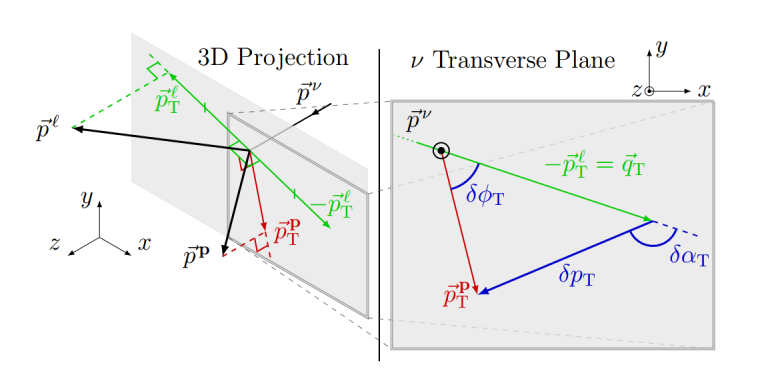
\includegraphics[width=\textwidth]{TalkPics/STVforHPTPC_101016/stvdiagram.png}
  \end{frame}

  \begin{frame}
    \frametitle{HPTPC Study}
    \begin{itemize}
    \item HPTPC-like and ND280-like momentum thresholds (below) and efficiencies (see Mark's talk) were applied to ND280 MC truth
    \item[-] Same as shown by Mark Scott previously
    \item Then calculated transverse variables
    \item[-] Only make sense in samples with a proton or a pion
    \item[-] CC0$\pi$Np, CC1$\pi$0p, CC1$\pi$Np
    \end{itemize}
    \begin{tabular}{l|cc}
      \hline
      Particle & ND280 Threshold/MeV & HPTPC Threshold/MeV \\
      \hline
      $\mu$ & 100 & 15 \\
      $\pi$ & 120 & 16 \\
      $p$ & 450 & 60 \\
      $e$ & 100 & 1 \\
      \hline
    \end{tabular}
  \end{frame}

  \begin{frame}
    \frametitle{HPTPC Study}
    \begin{itemize}
    \item Will show the $\delta\alpha_{T}$, $\delta\phi_{T}$ and $\delta p_{T}$ for all four samples
    \item[-] apologies for large number of plots
    \item Will show both ND280 and HPTPC thresholds and efficiencies
    \item Truth information is used to determine which events truly belong in the sample (``correct''), and which are fakes (``false'')
    \item[-] Distributions of transverse variables are shown for both
    \end{itemize}
  \end{frame}

  \begin{frame}
    \frametitle{CC0$\pi$NP}
    \centering
    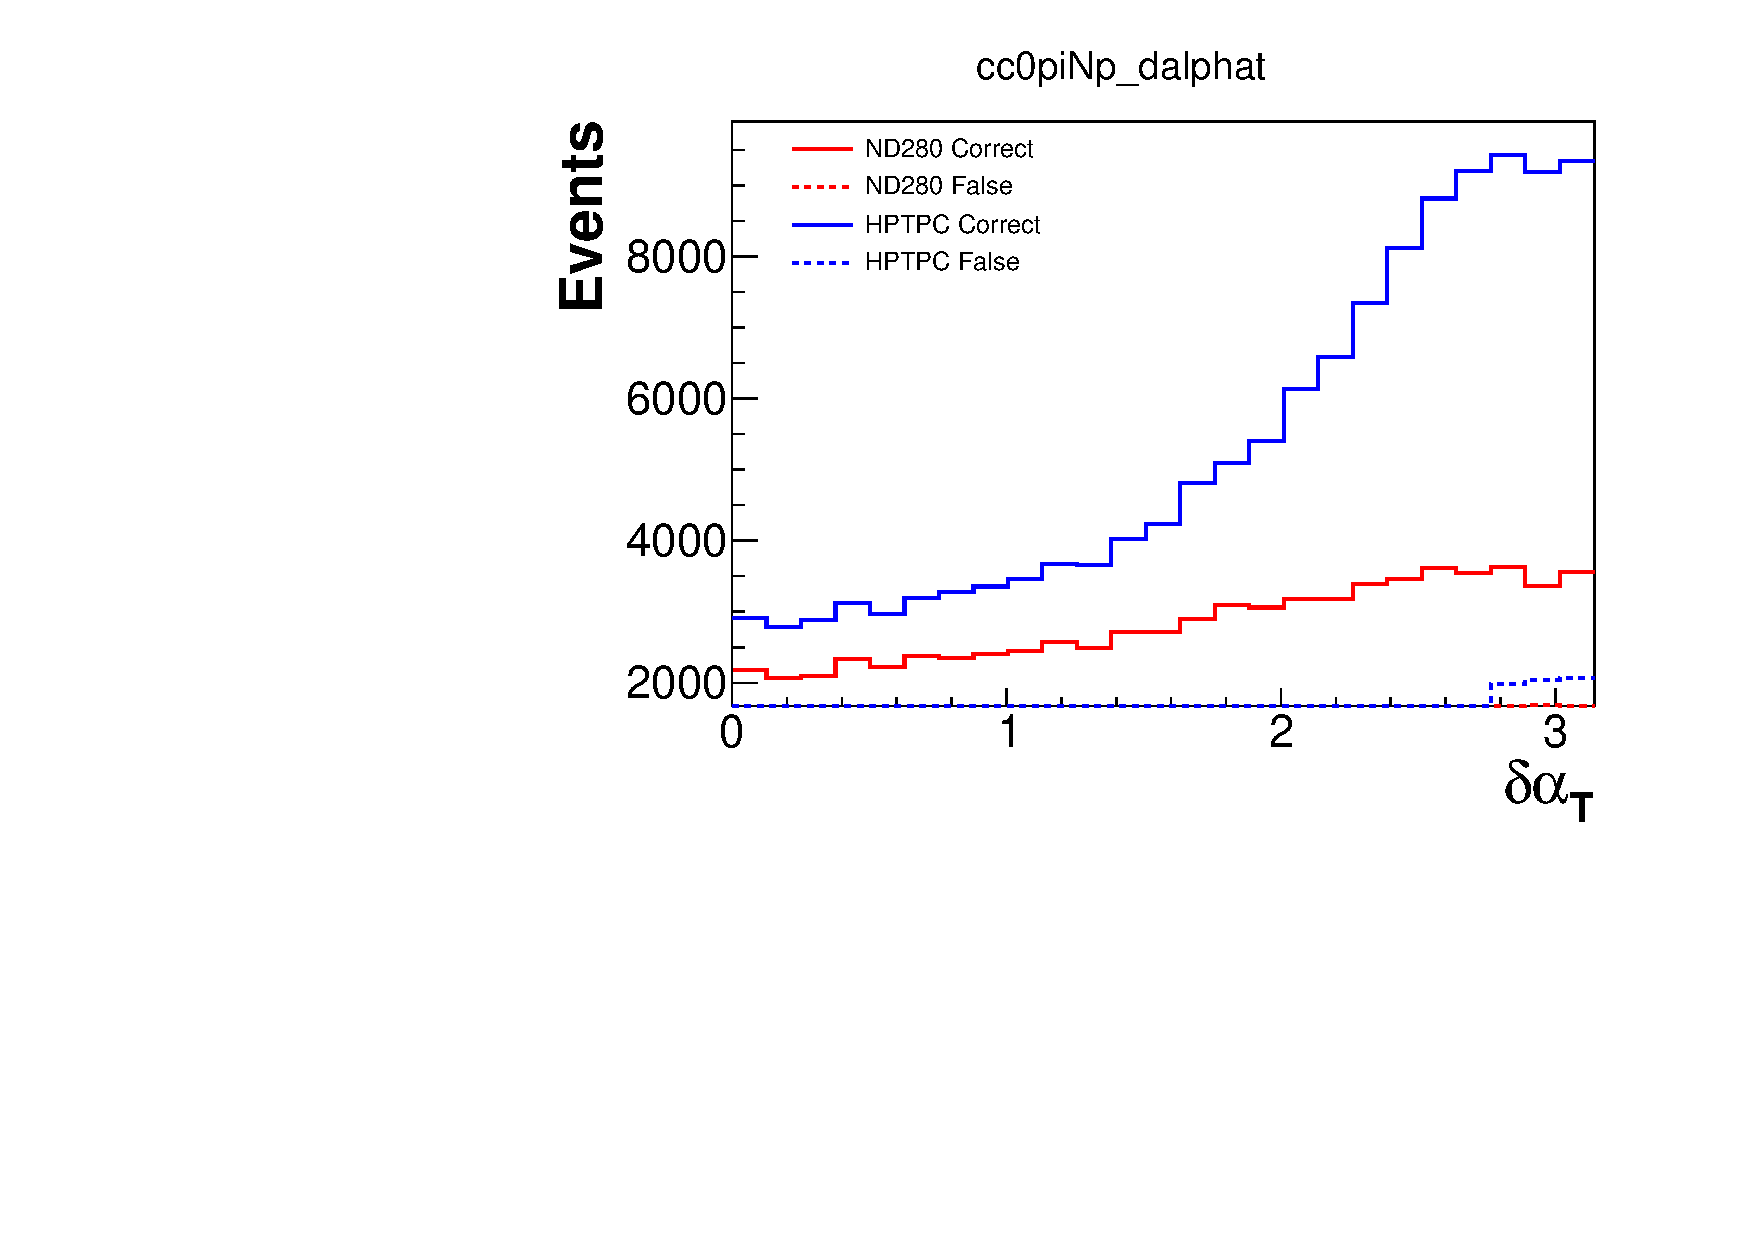
\includegraphics[width=.47\textwidth]{TalkPics/STVforHPTPC_101016/plots/cc0piNp_dalphat.pdf}
    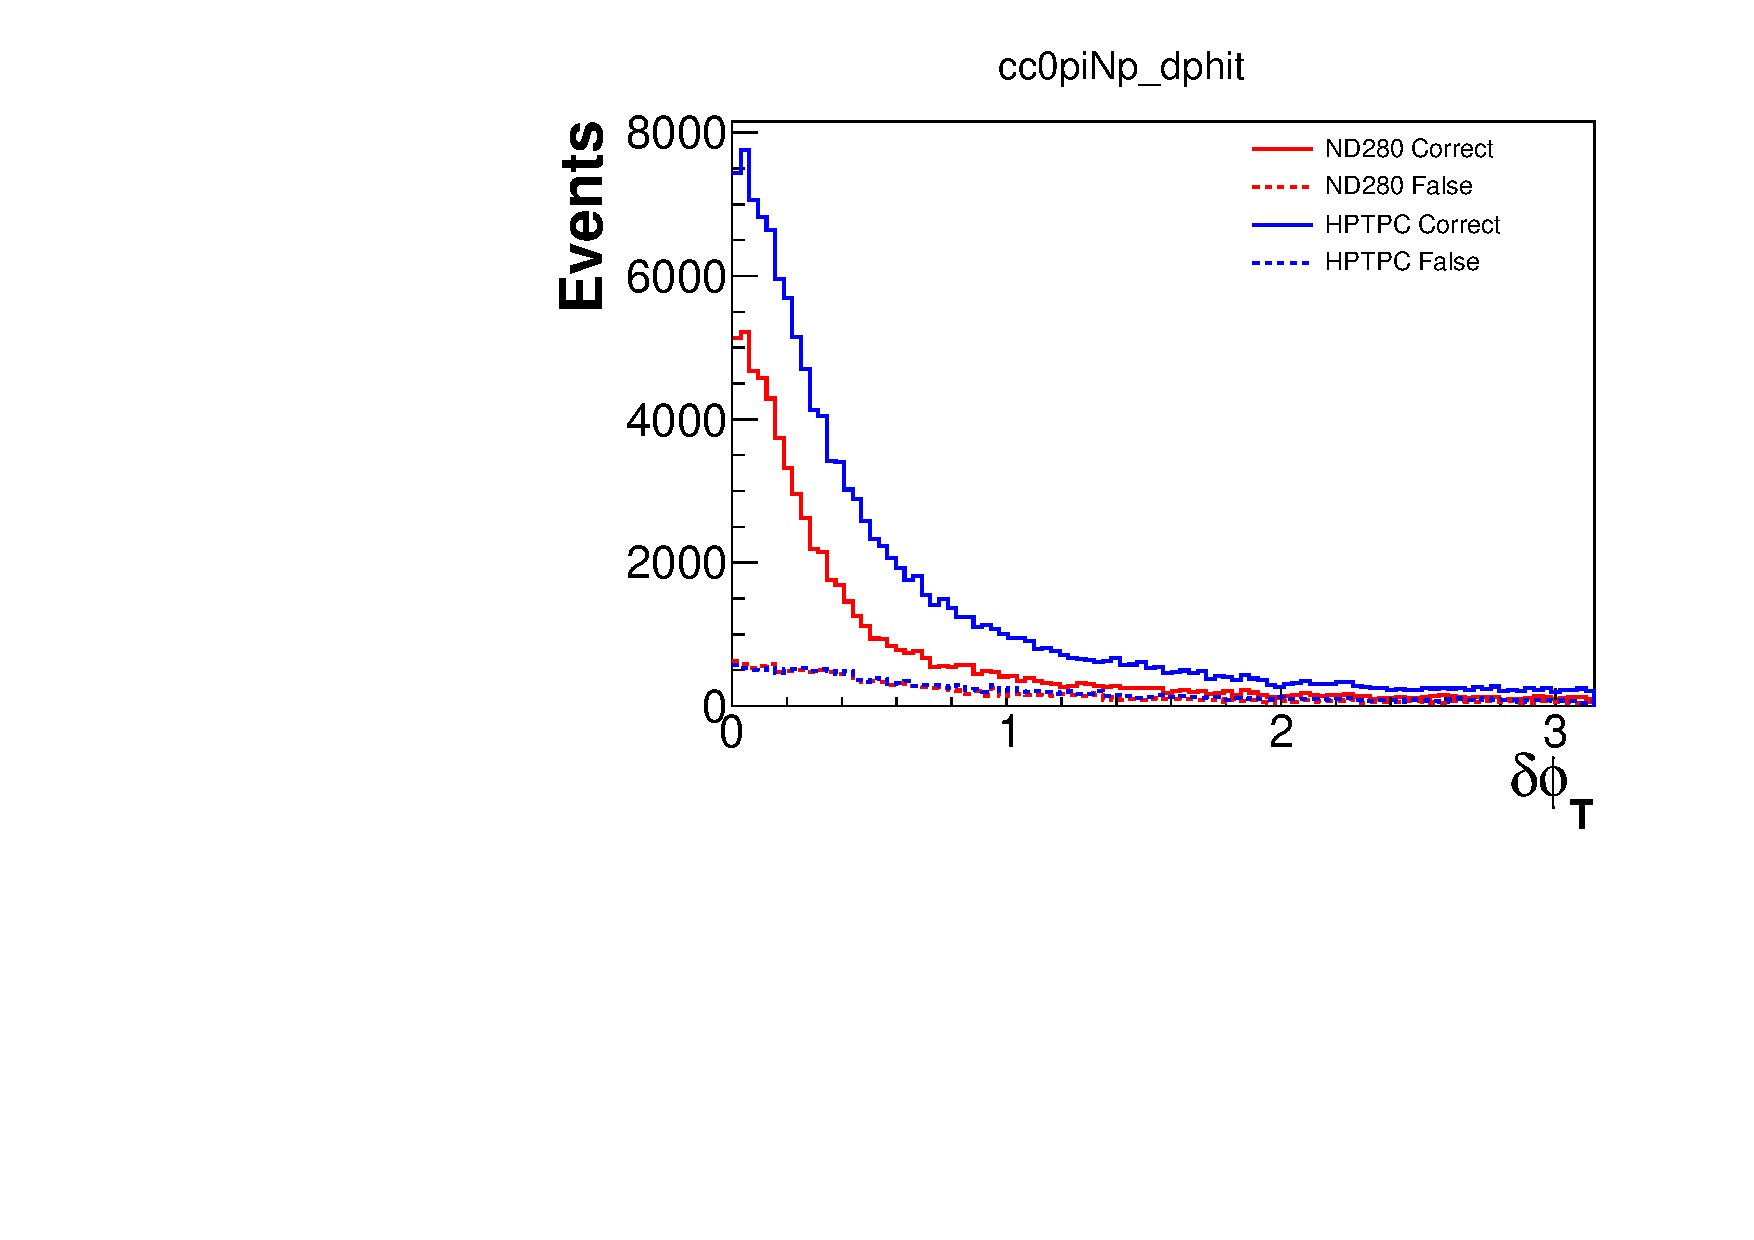
\includegraphics[width=.47\textwidth]{TalkPics/STVforHPTPC_101016/plots/cc0piNp_dphit.pdf}

    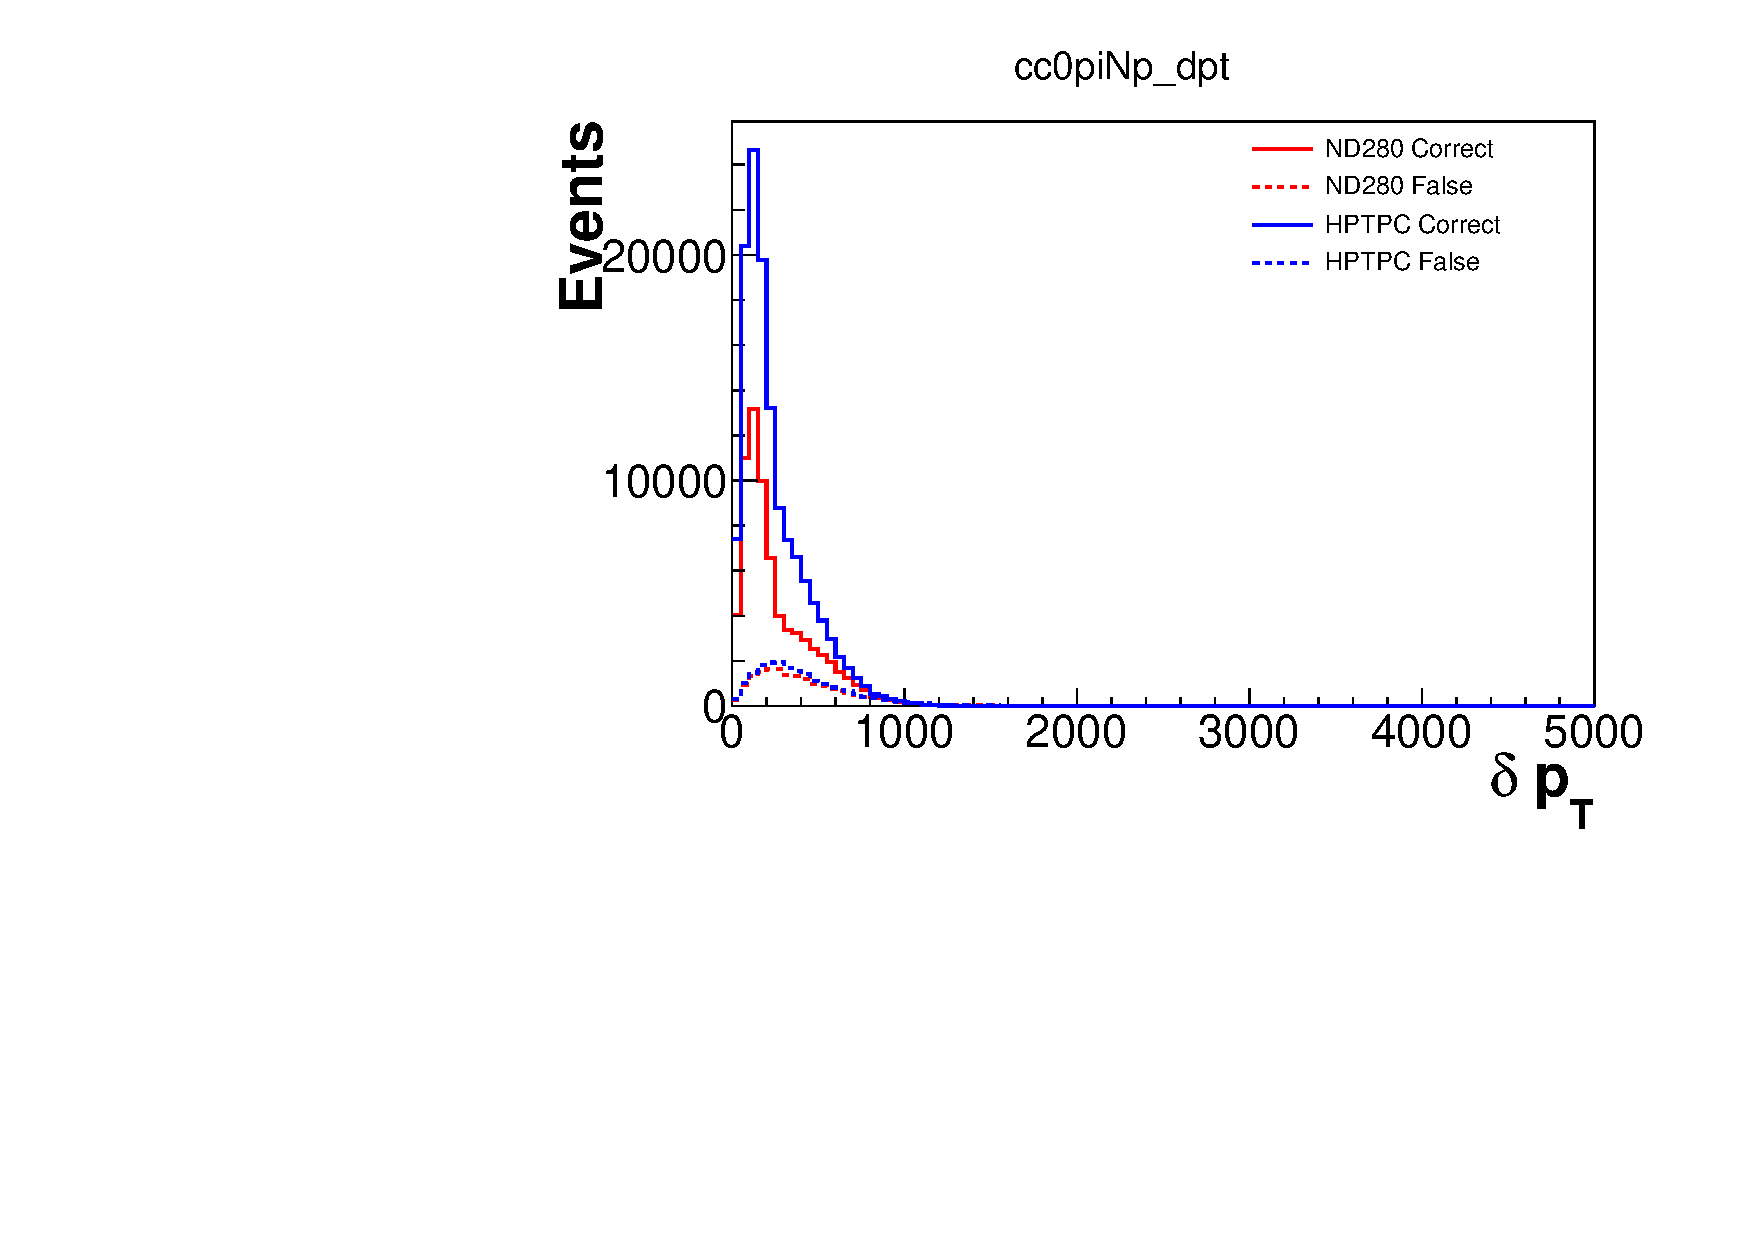
\includegraphics[width=.47\textwidth]{TalkPics/STVforHPTPC_101016/plots/cc0piNp_dpt.pdf}
  \end{frame}

  \begin{frame}
    \frametitle{CC0$\pi$NP}
    \centering
    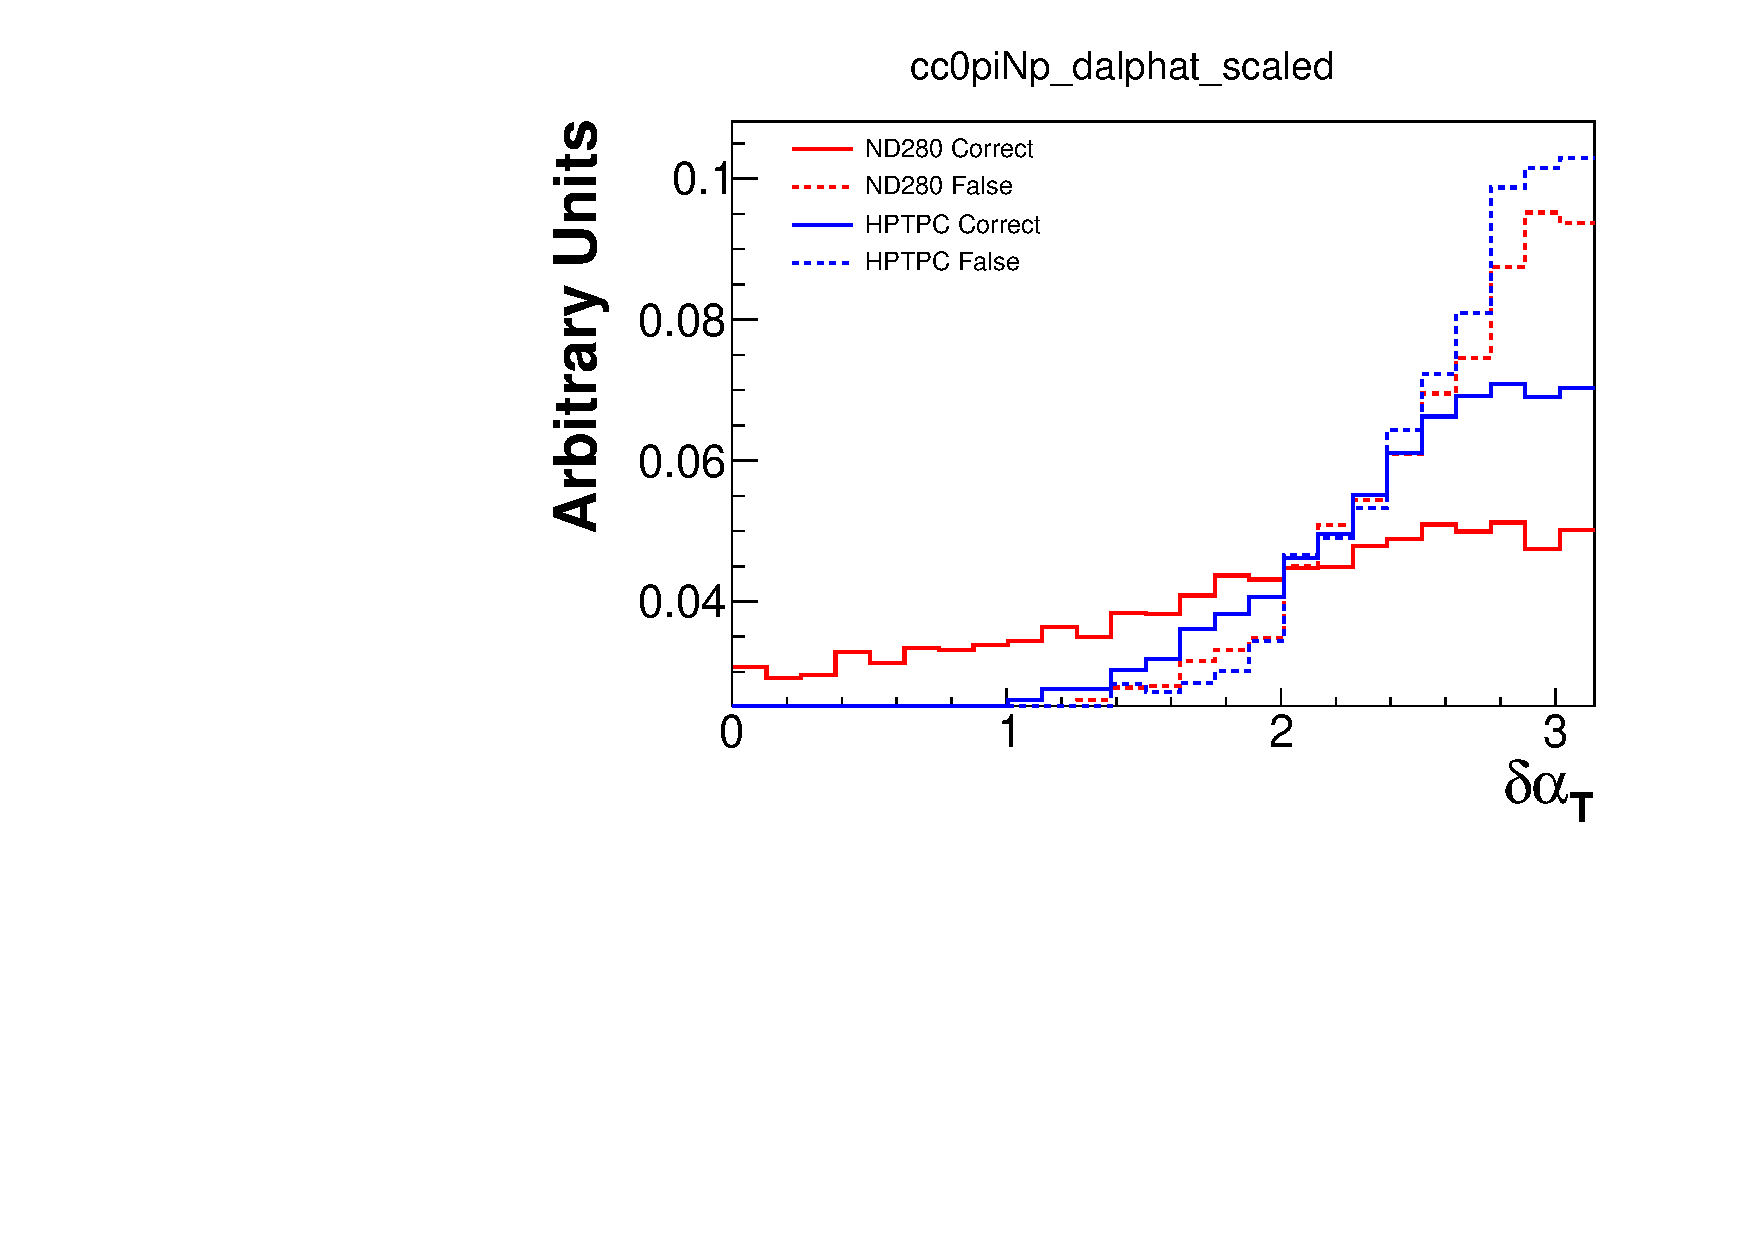
\includegraphics[width=.47\textwidth]{TalkPics/STVforHPTPC_101016/plots/cc0piNp_dalphat_scaled.pdf}
    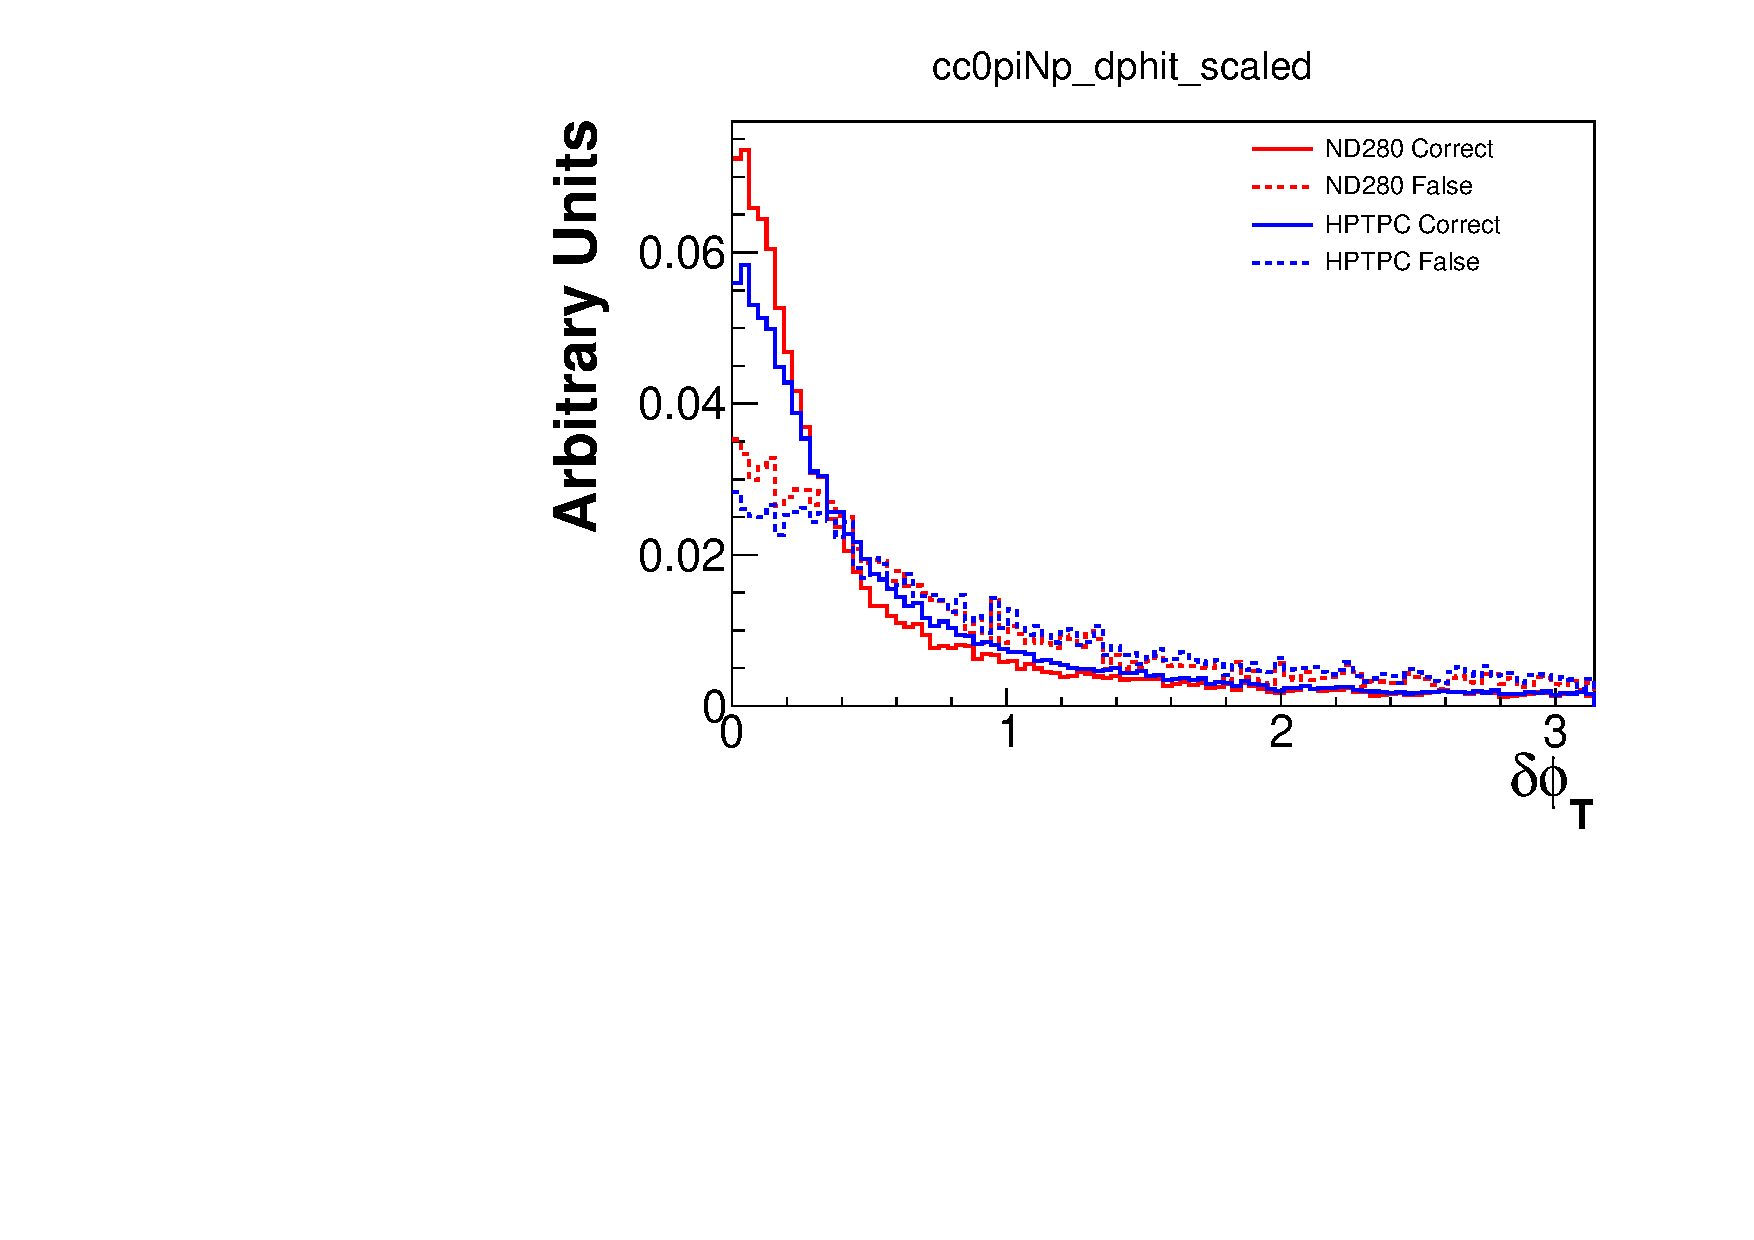
\includegraphics[width=.47\textwidth]{TalkPics/STVforHPTPC_101016/plots/cc0piNp_dphit_scaled.pdf}

    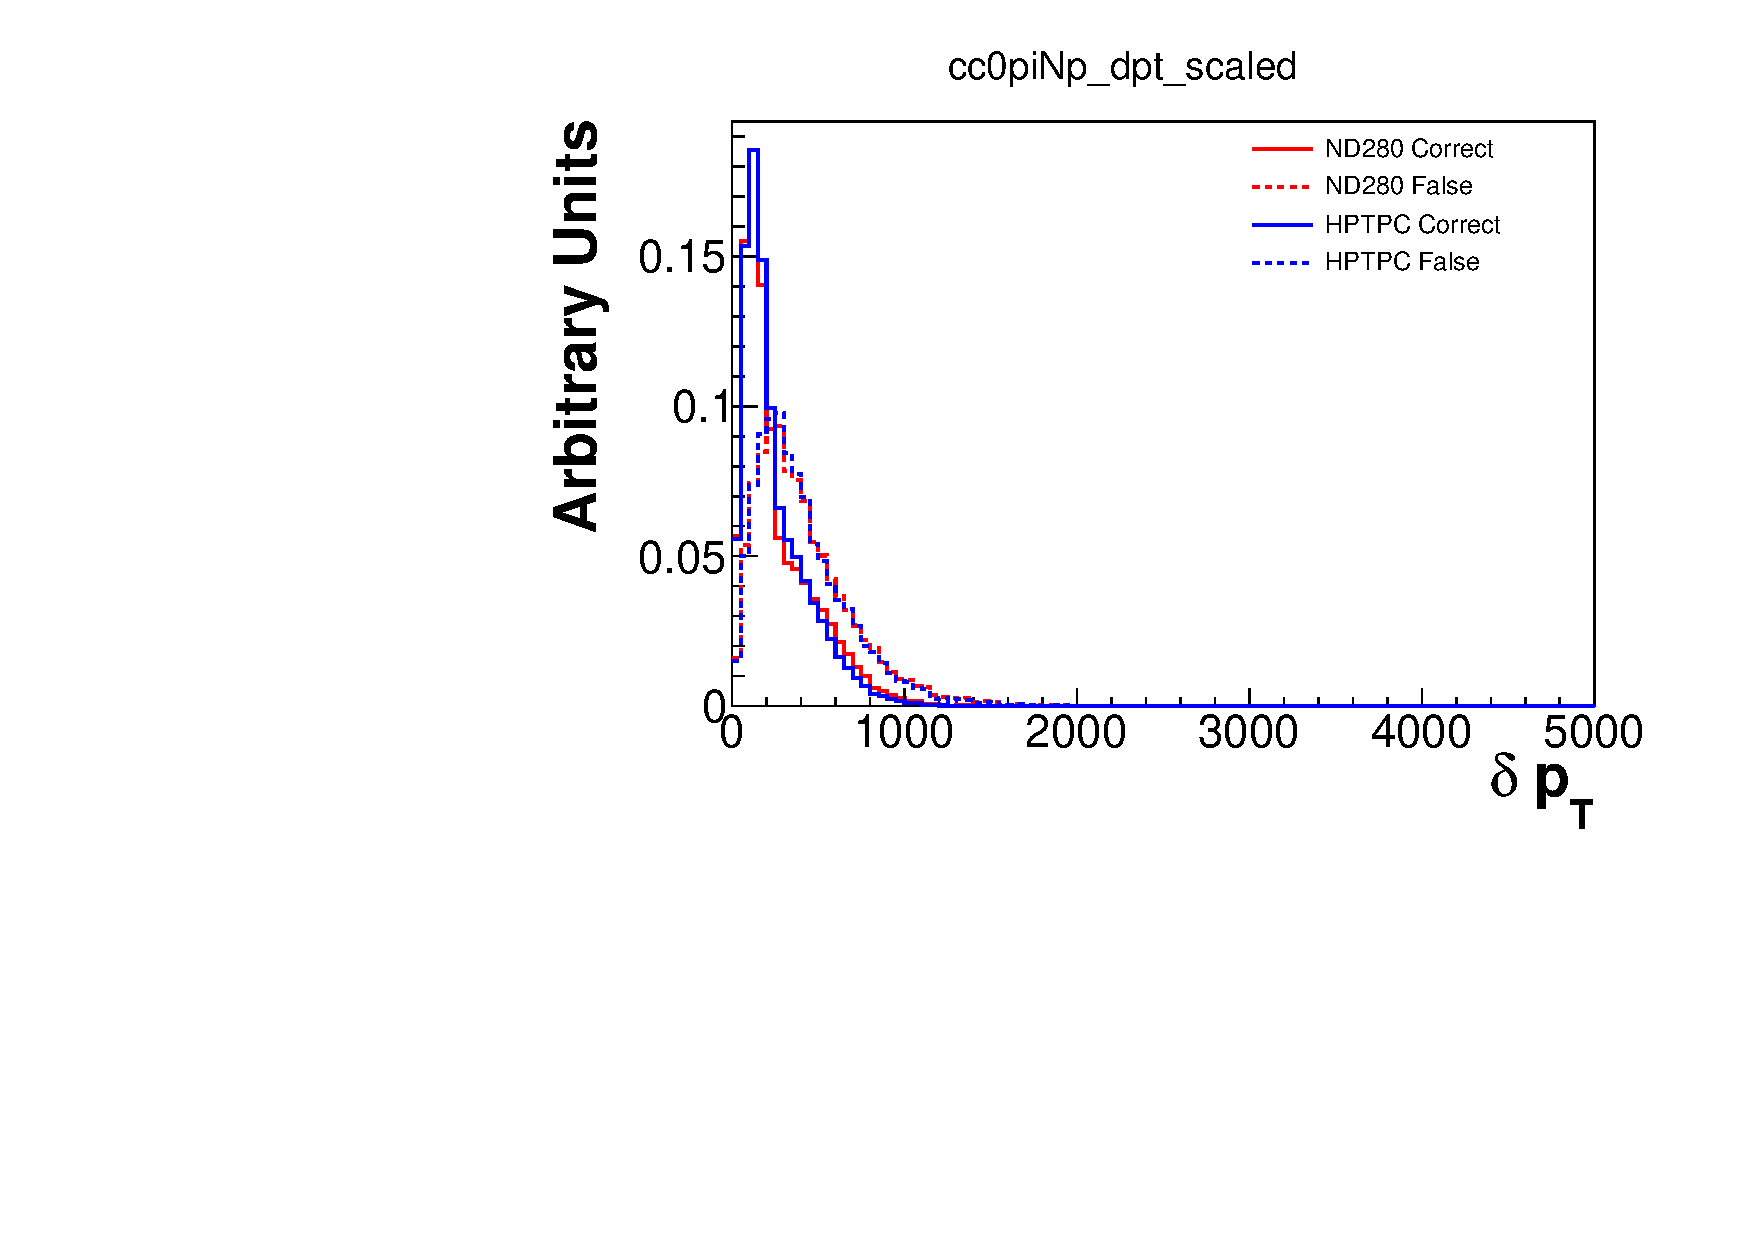
\includegraphics[width=.47\textwidth]{TalkPics/STVforHPTPC_101016/plots/cc0piNp_dpt_scaled.pdf}
  \end{frame}

  \begin{frame}
    \frametitle{CC1$\pi$0P}
    \centering
    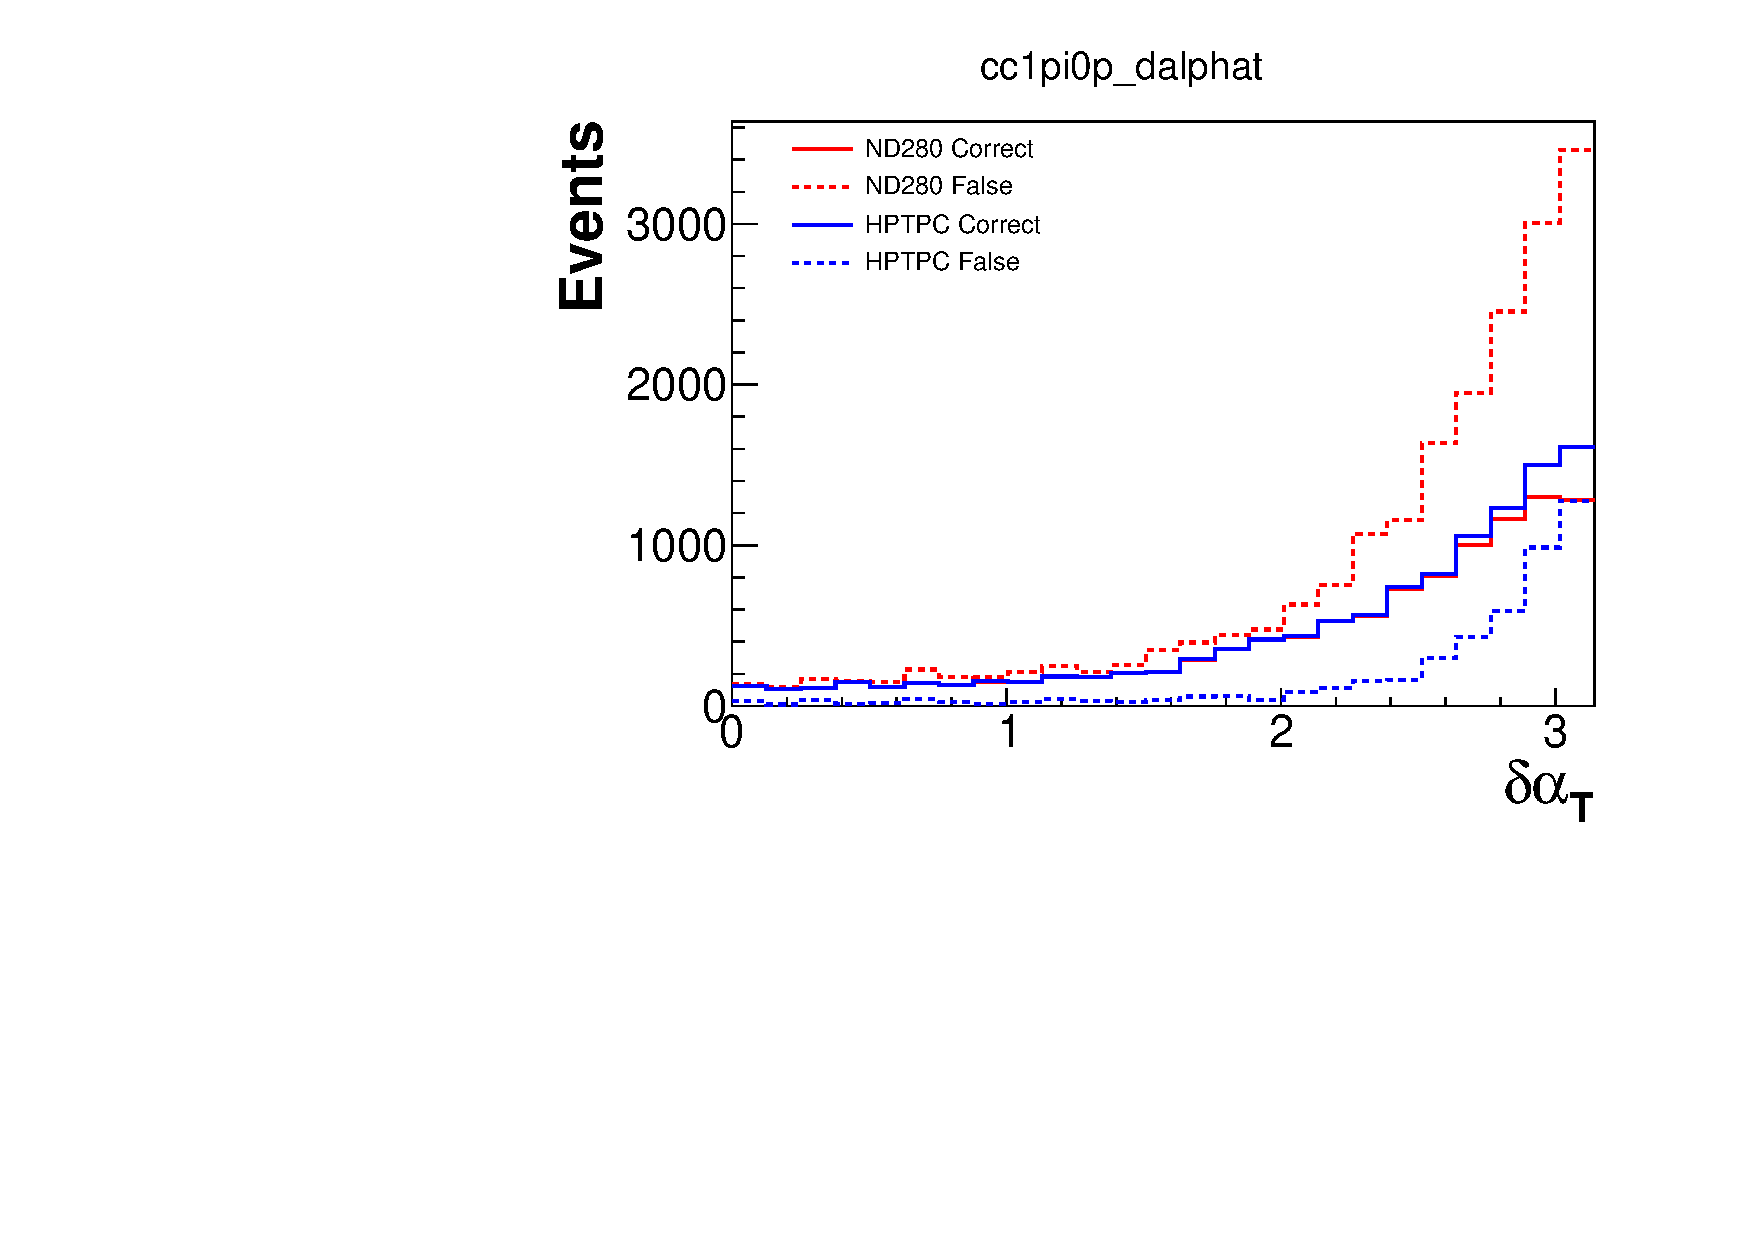
\includegraphics[width=.47\textwidth]{TalkPics/STVforHPTPC_101016/plots/cc1pi0p_dalphat.pdf}
    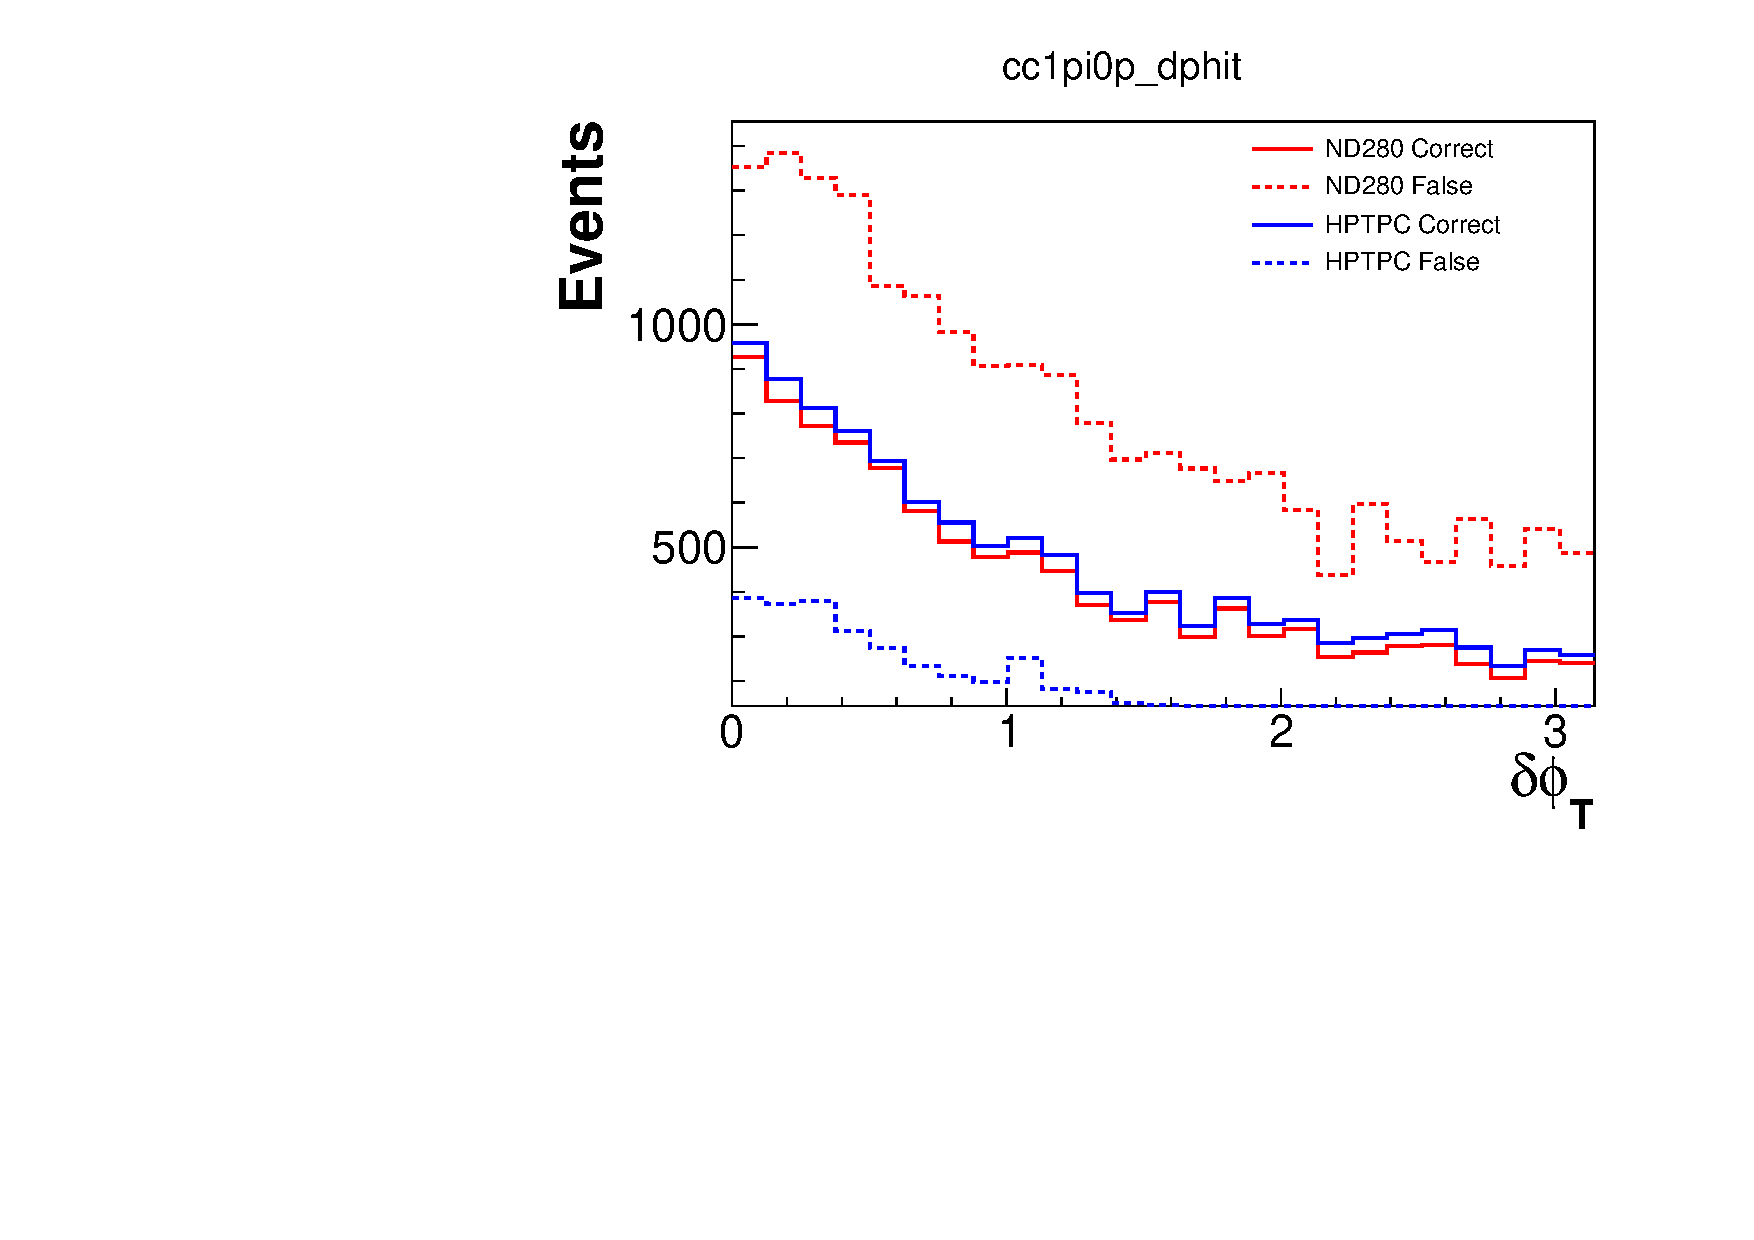
\includegraphics[width=.47\textwidth]{TalkPics/STVforHPTPC_101016/plots/cc1pi0p_dphit.pdf}

    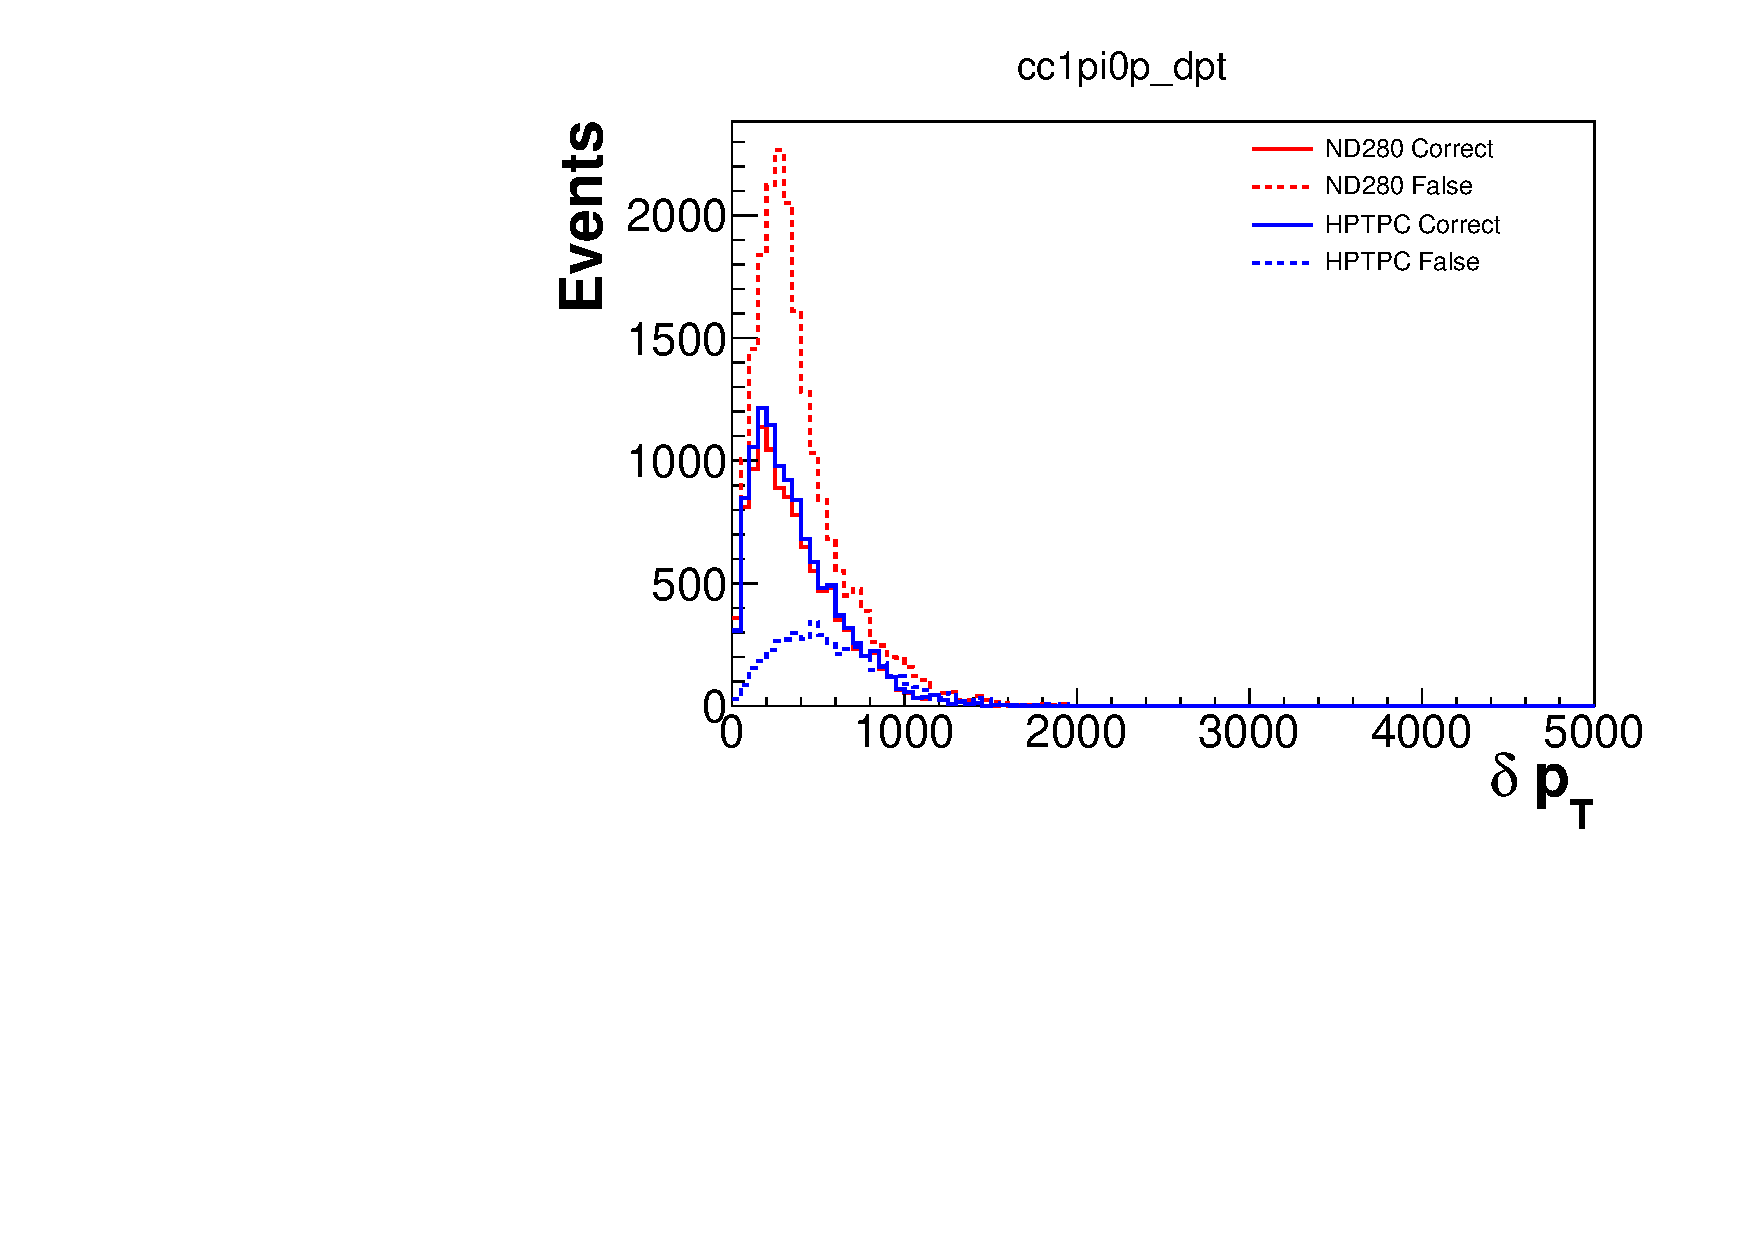
\includegraphics[width=.47\textwidth]{TalkPics/STVforHPTPC_101016/plots/cc1pi0p_dpt.pdf}
  \end{frame}

  \begin{frame}
    \frametitle{CC1$\pi$0P}
    \centering
    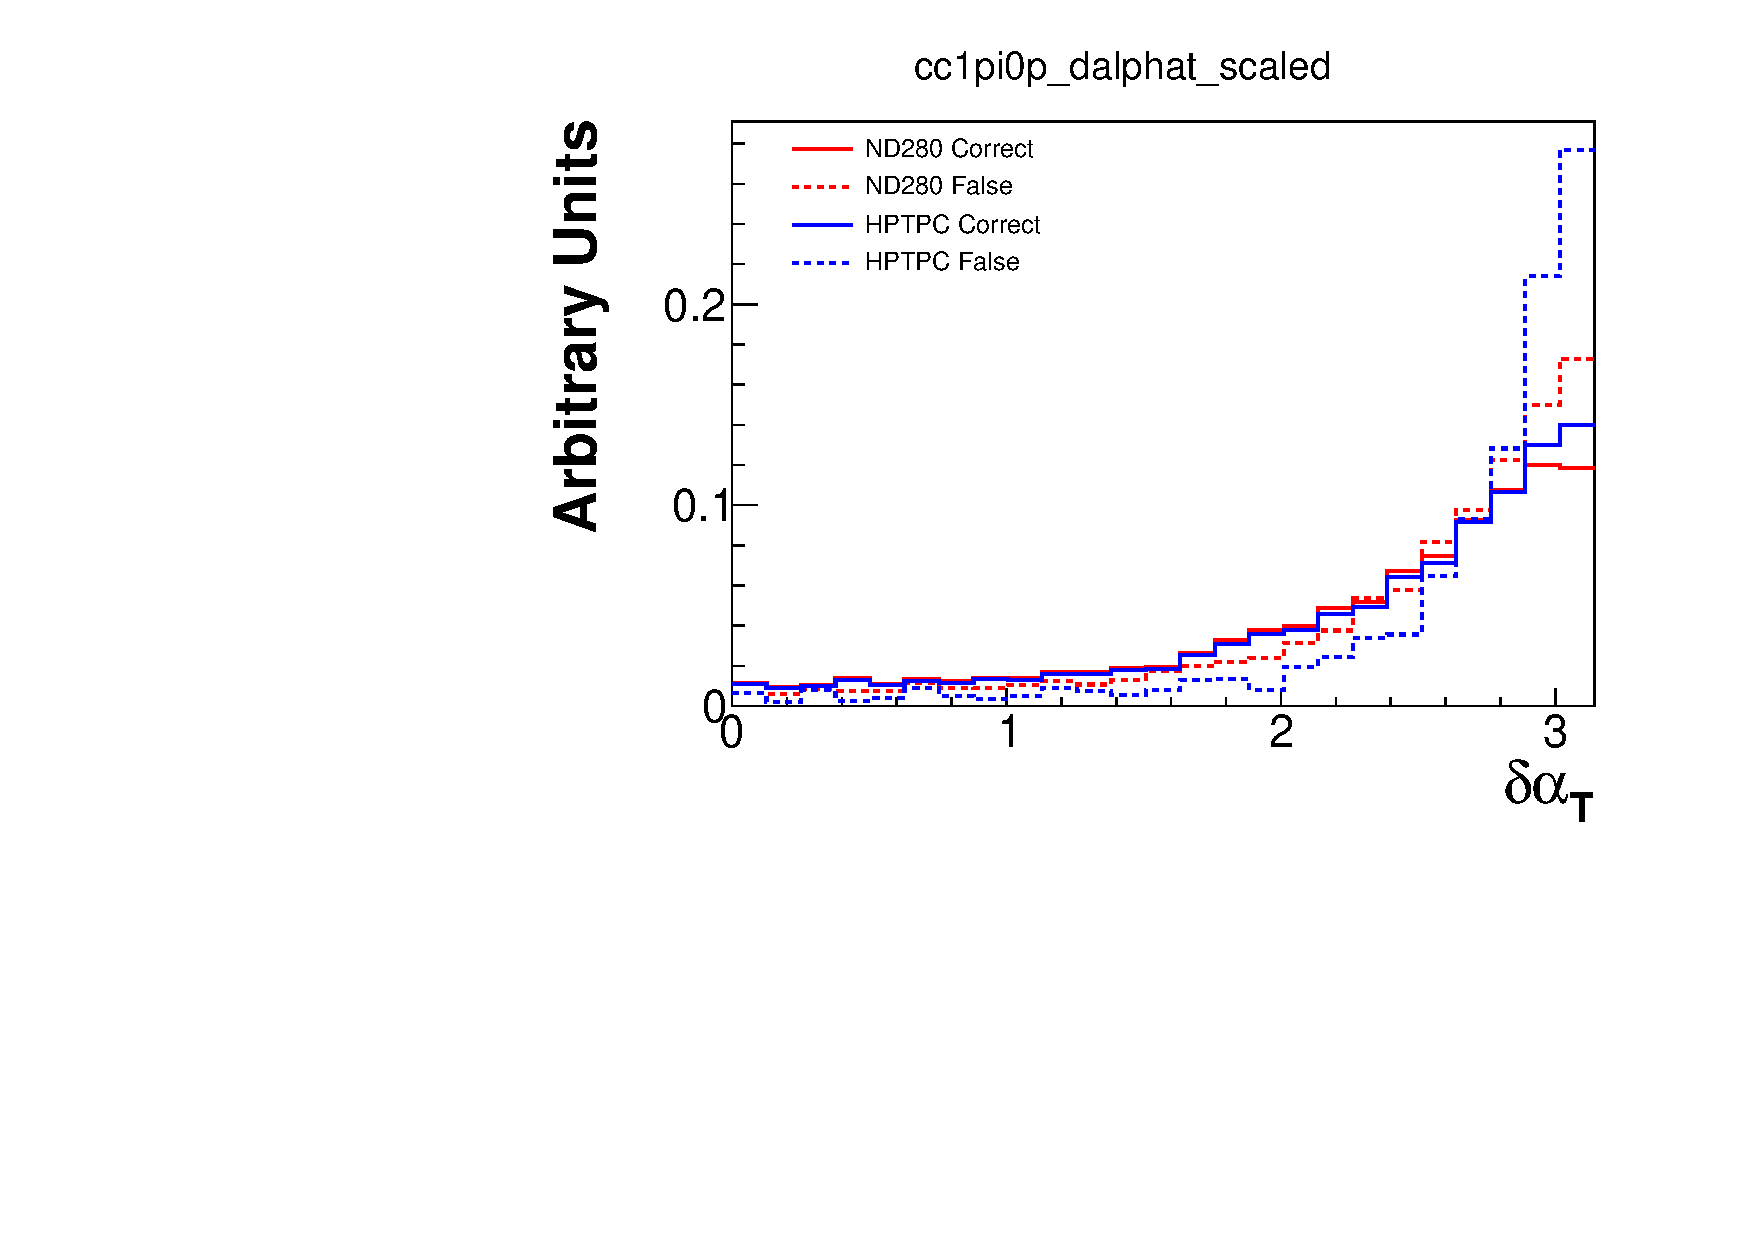
\includegraphics[width=.47\textwidth]{TalkPics/STVforHPTPC_101016/plots/cc1pi0p_dalphat_scaled.pdf}
    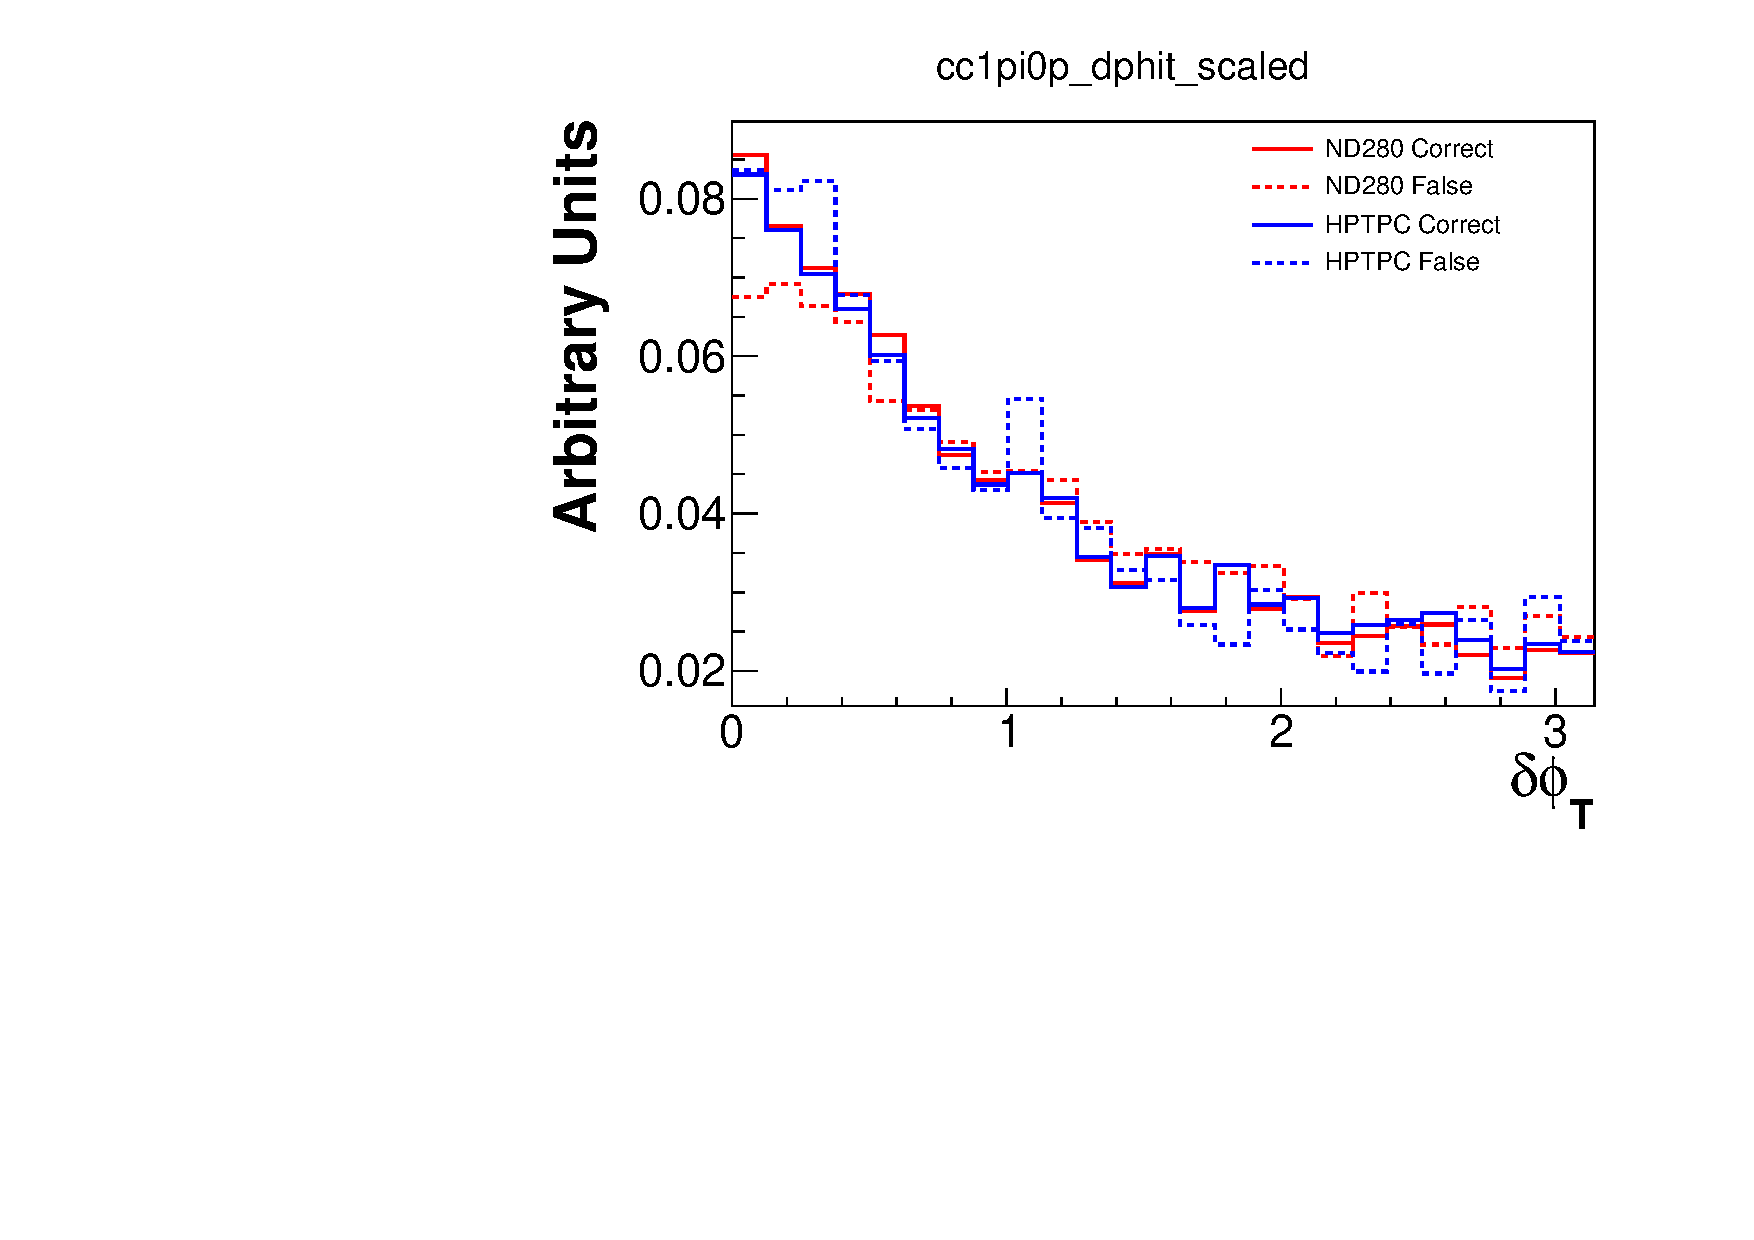
\includegraphics[width=.47\textwidth]{TalkPics/STVforHPTPC_101016/plots/cc1pi0p_dphit_scaled.pdf}

    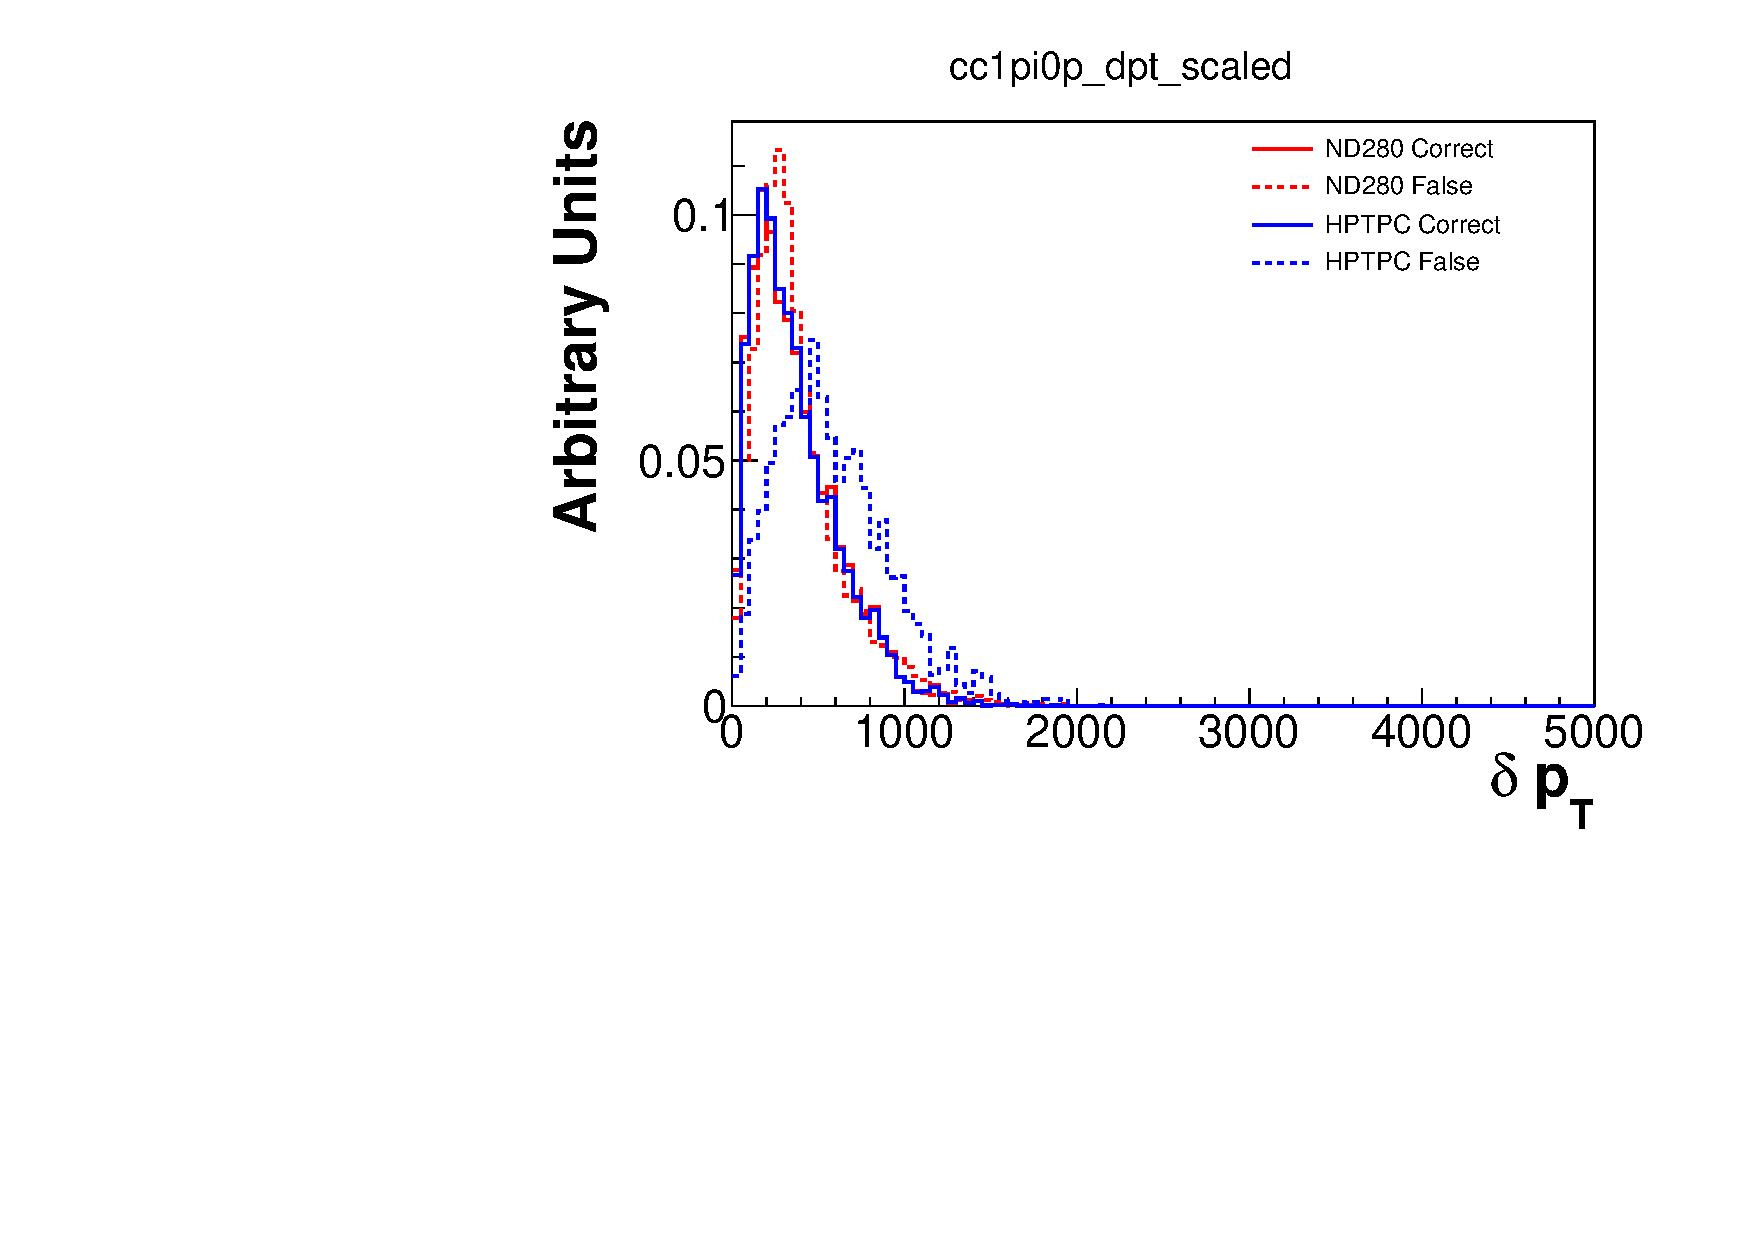
\includegraphics[width=.47\textwidth]{TalkPics/STVforHPTPC_101016/plots/cc1pi0p_dpt_scaled.pdf}
  \end{frame}

  \begin{frame}
    \frametitle{CC1$\pi$0P - difference hypothesis}
    \vspace{-.2cm}
    \begin{itemize}
    \item Pion threshold is much lower in HPTPC (120 vs 16 MeV)
    \item Therefore HPTPC sample contains more $p$+$\pi$ events where the proton is missed and the pion is of low energy
    \item Increases the number of false events with high $\delta p_{T}$ and $\delta\alpha_{T}$
    \item Will investigate 2D distributions of events
    \end{itemize}
    \vspace{-.2cm}
    \centering
    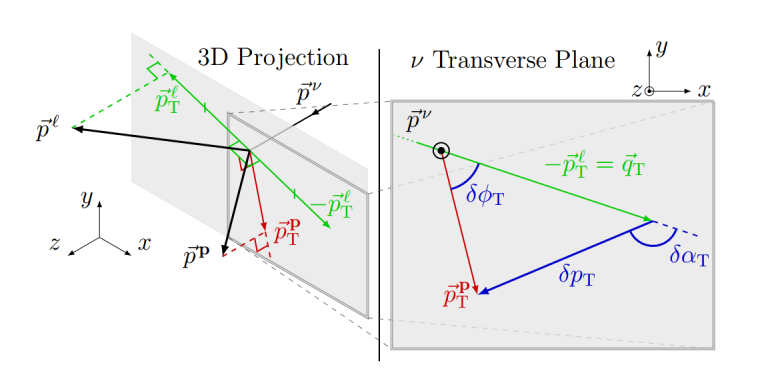
\includegraphics[width=.9\textwidth]{TalkPics/STVforHPTPC_101016/stvdiagram.png}
  \end{frame}

  \begin{frame}
    \frametitle{CC1$\pi$NP}
    \centering
    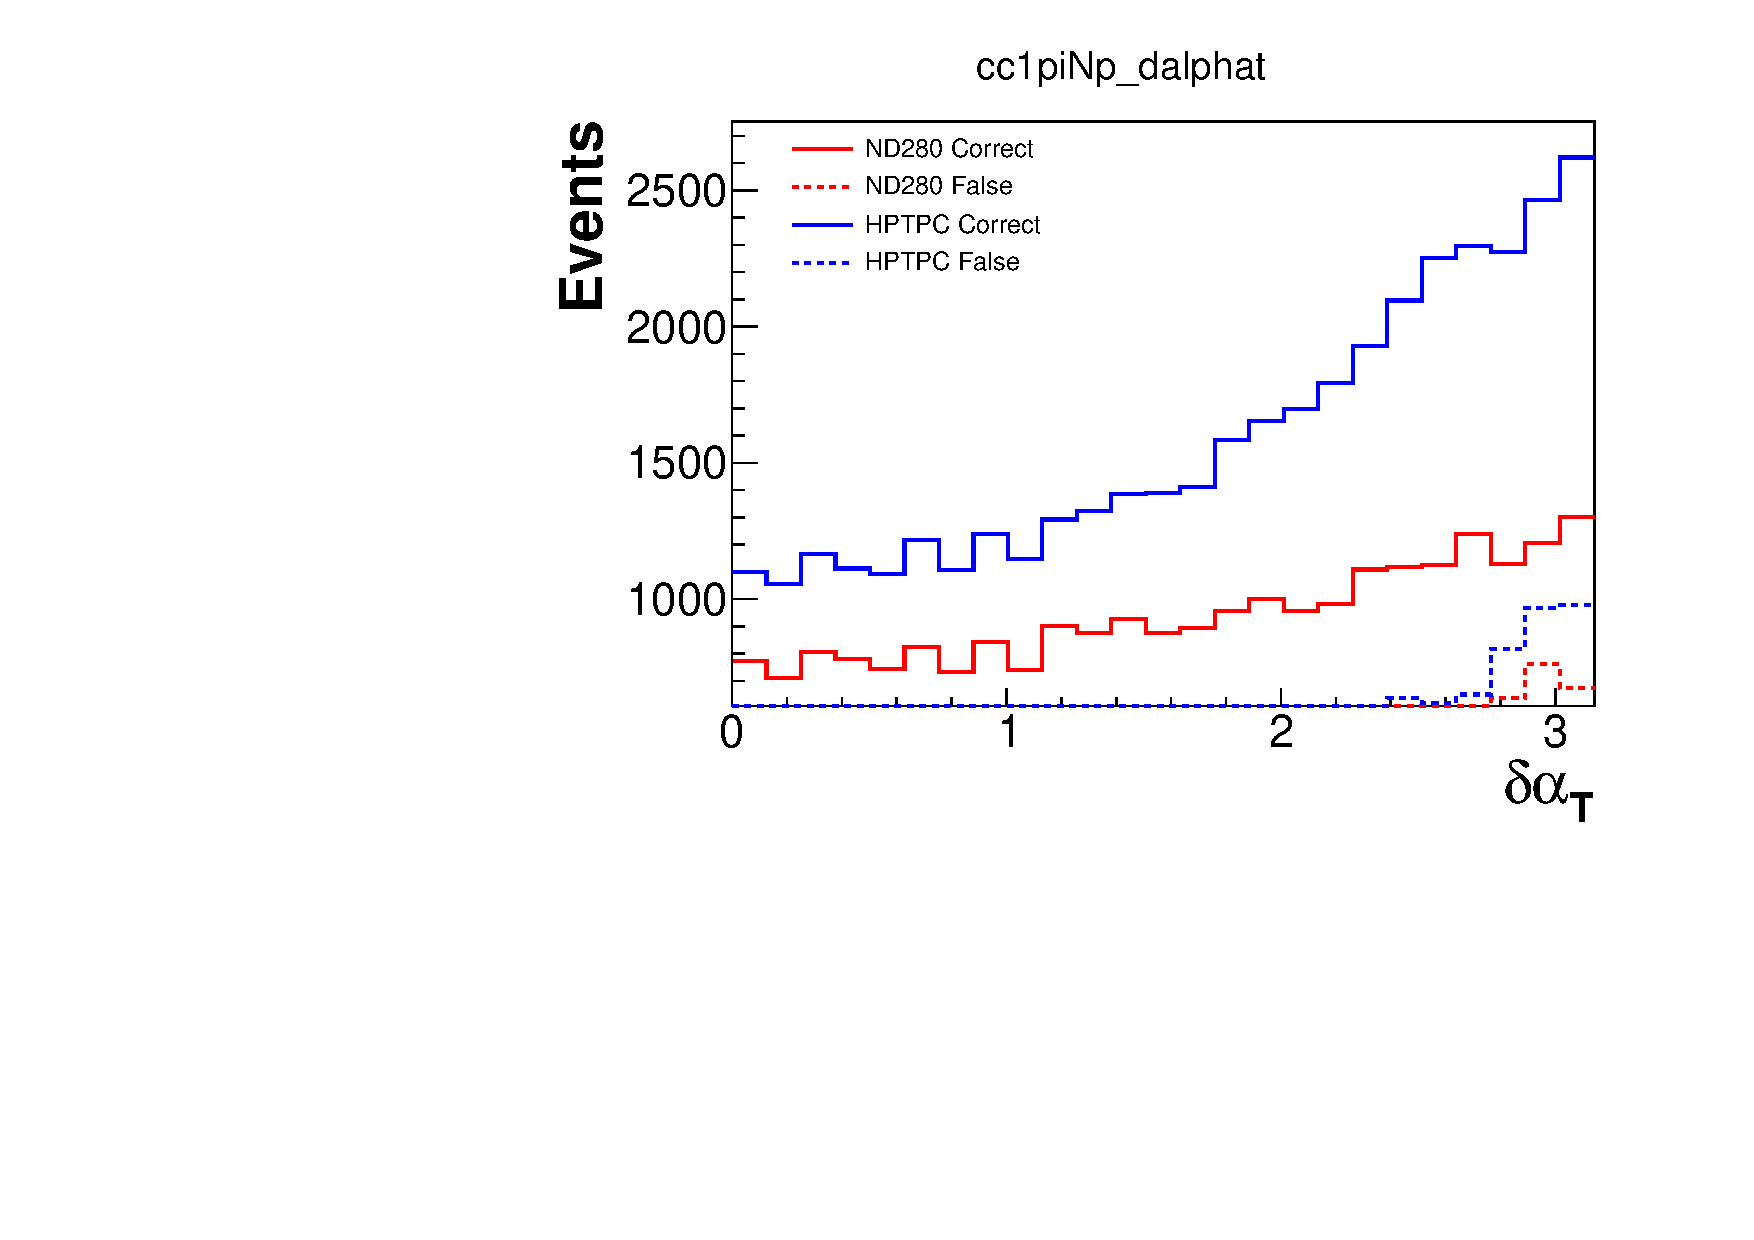
\includegraphics[width=.47\textwidth]{TalkPics/STVforHPTPC_101016/plots/cc1piNp_dalphat.pdf}
    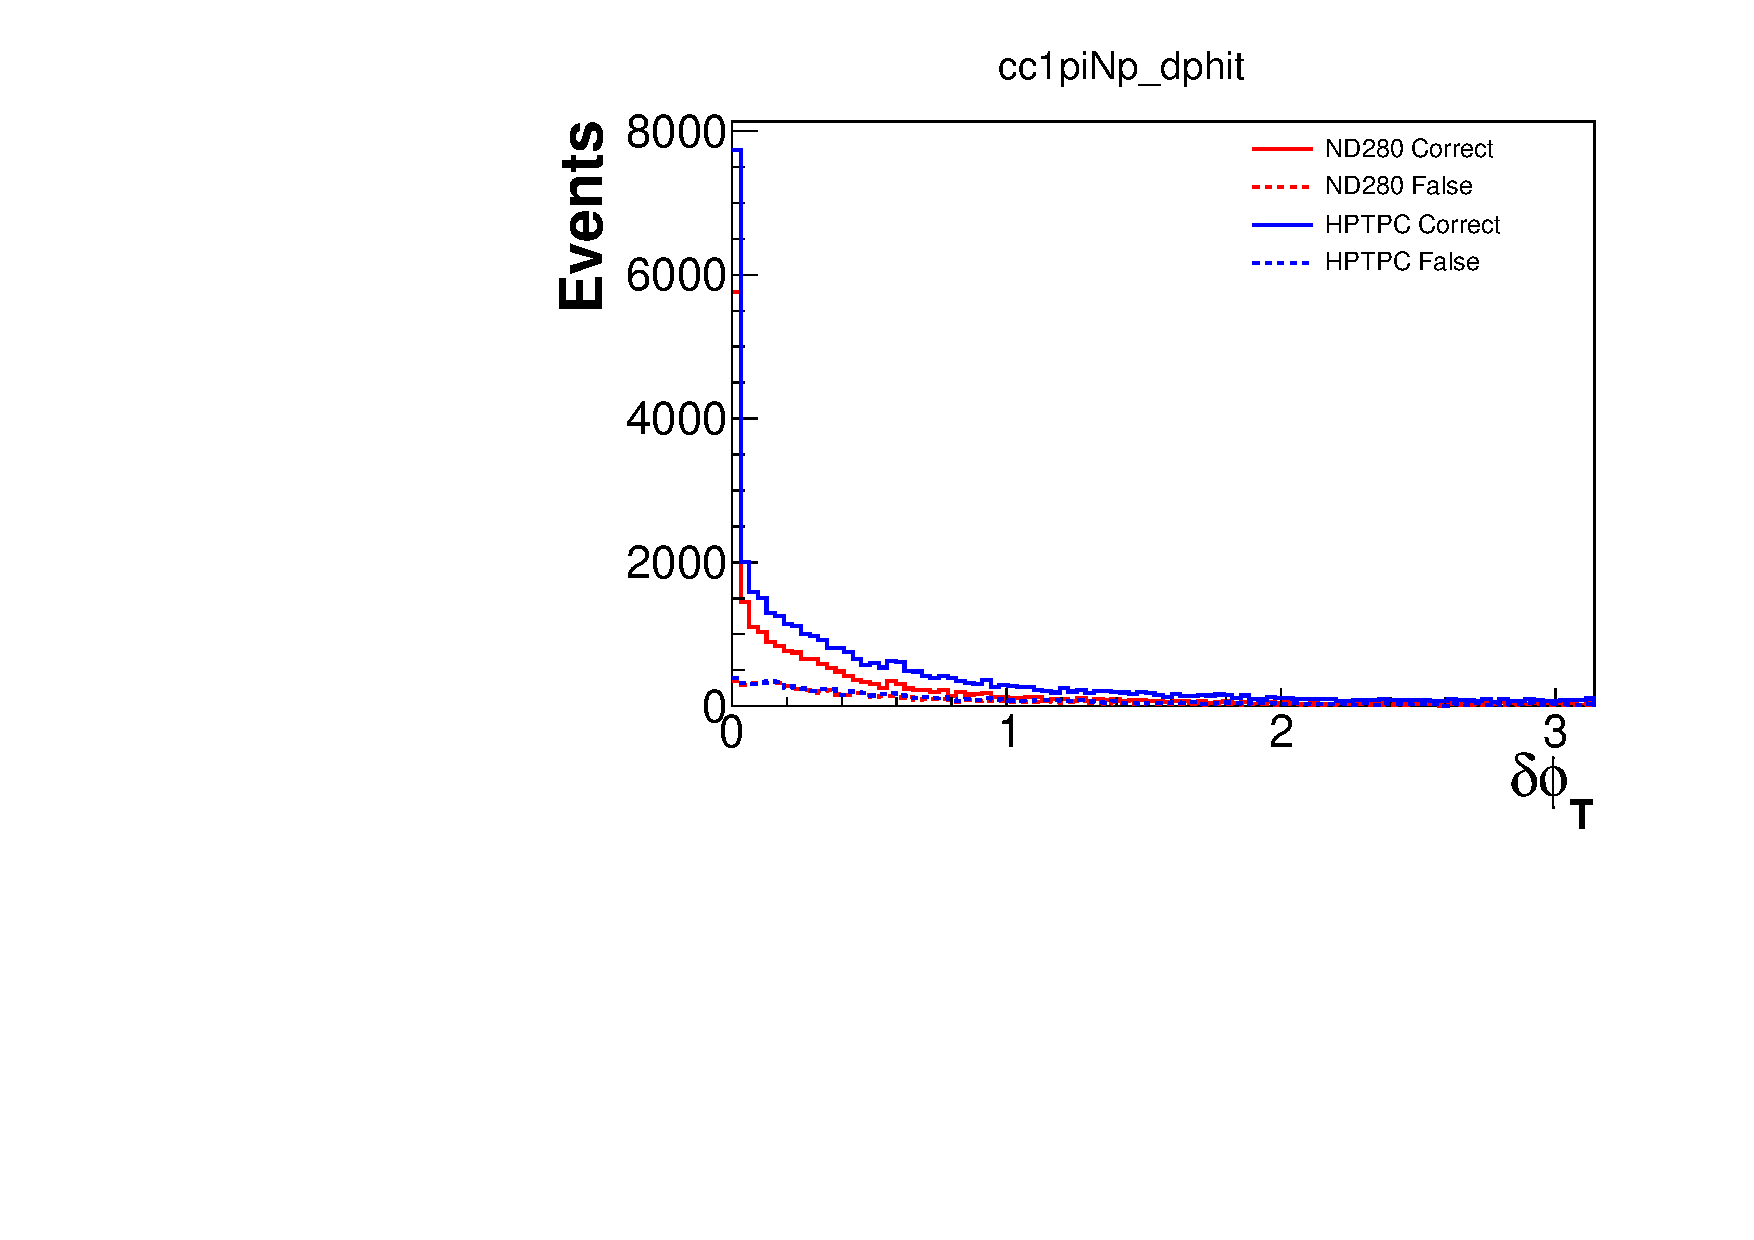
\includegraphics[width=.47\textwidth]{TalkPics/STVforHPTPC_101016/plots/cc1piNp_dphit.pdf}

    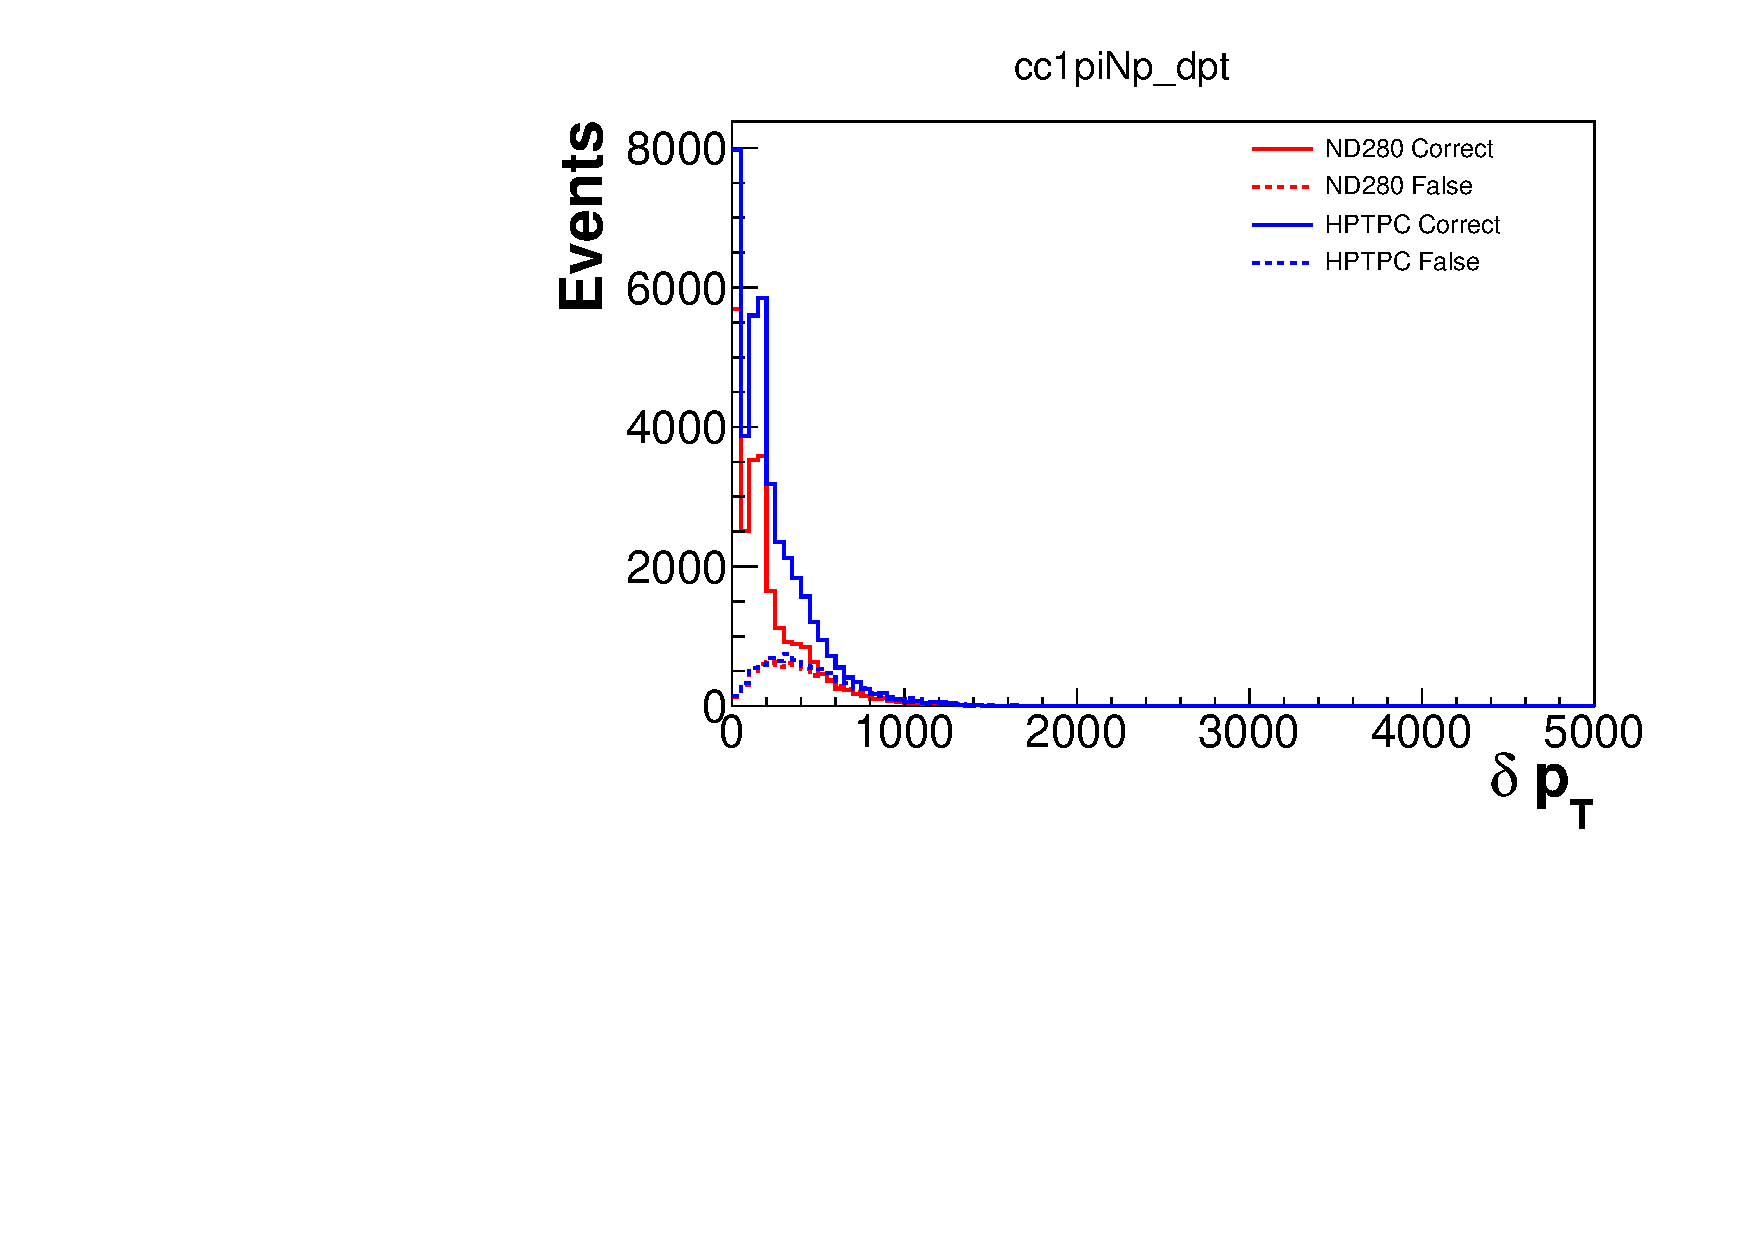
\includegraphics[width=.47\textwidth]{TalkPics/STVforHPTPC_101016/plots/cc1piNp_dpt.pdf}
  \end{frame}

  \begin{frame}
    \frametitle{CC1$\pi$NP}
    \centering
    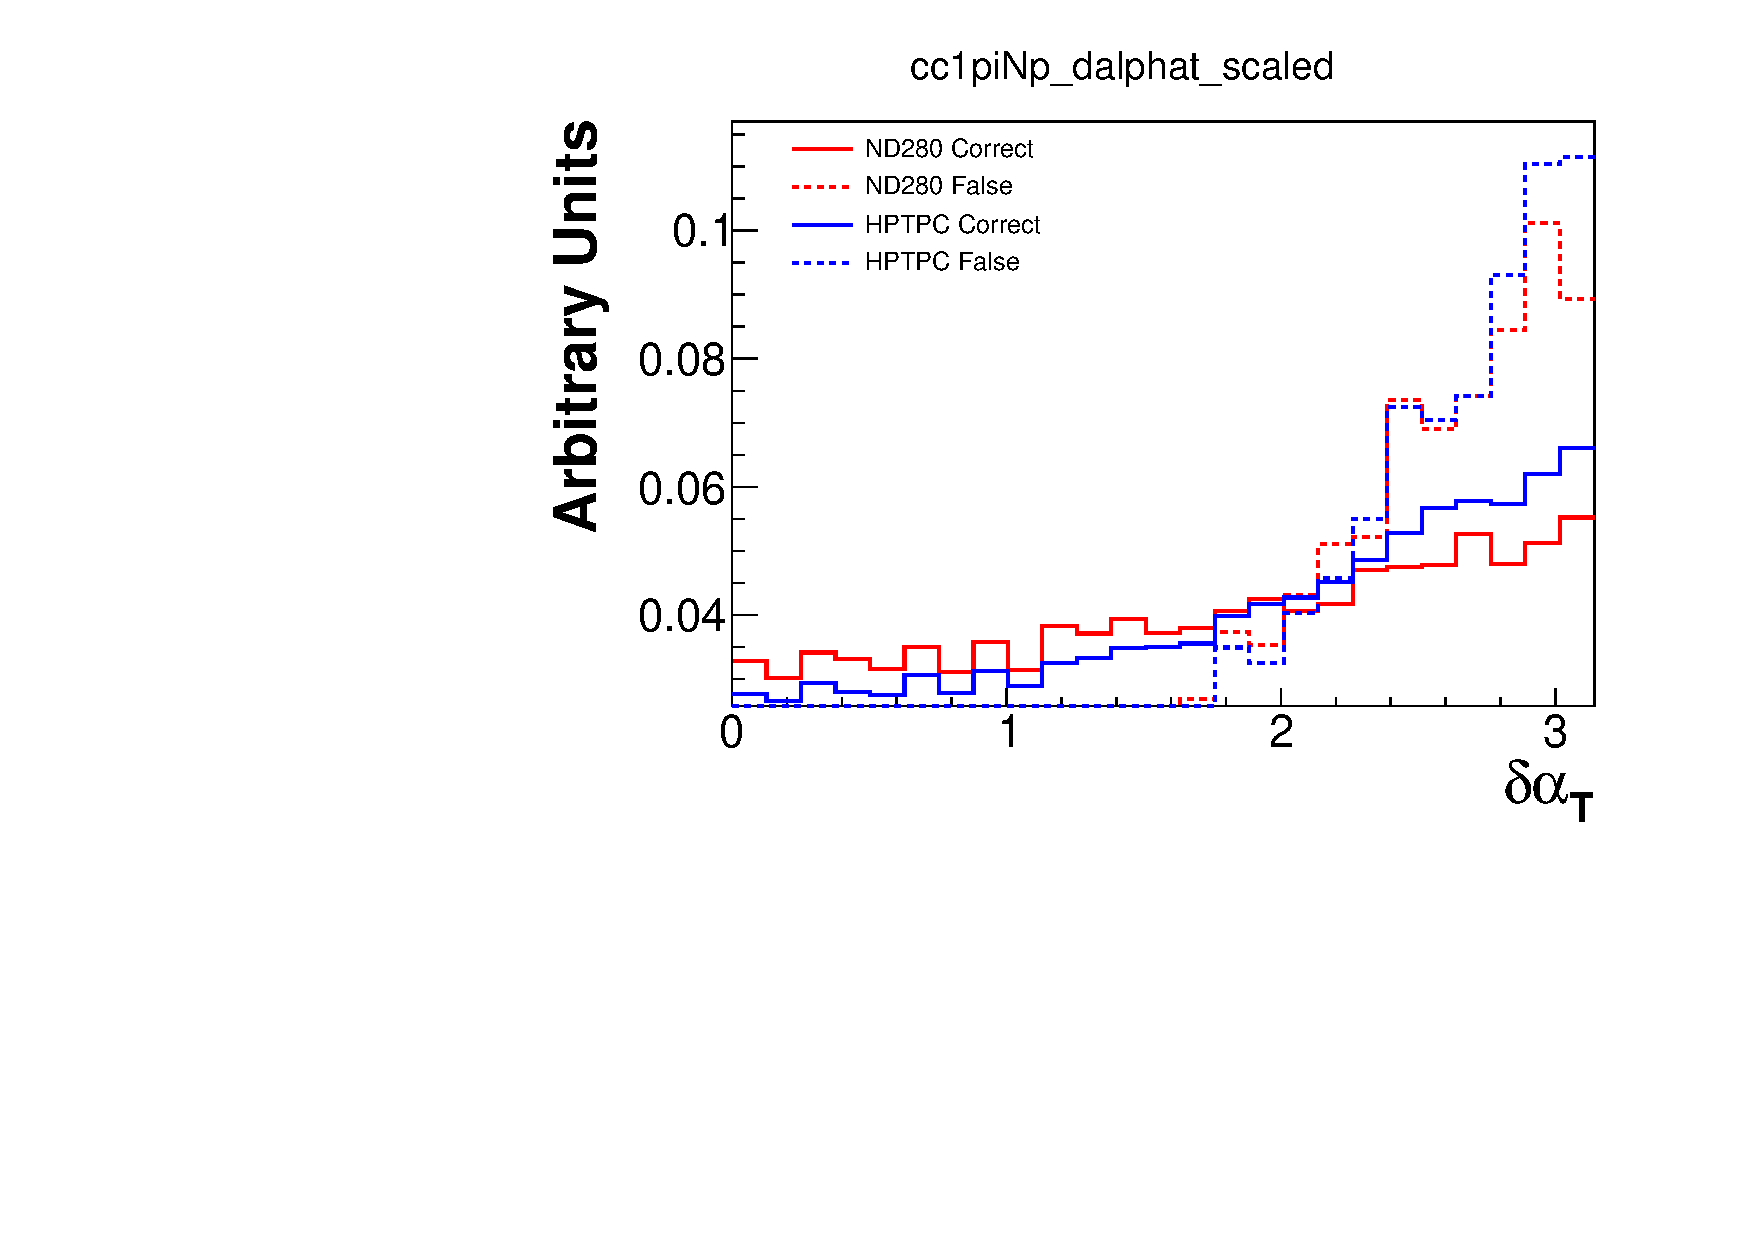
\includegraphics[width=.47\textwidth]{TalkPics/STVforHPTPC_101016/plots/cc1piNp_dalphat_scaled.pdf}
    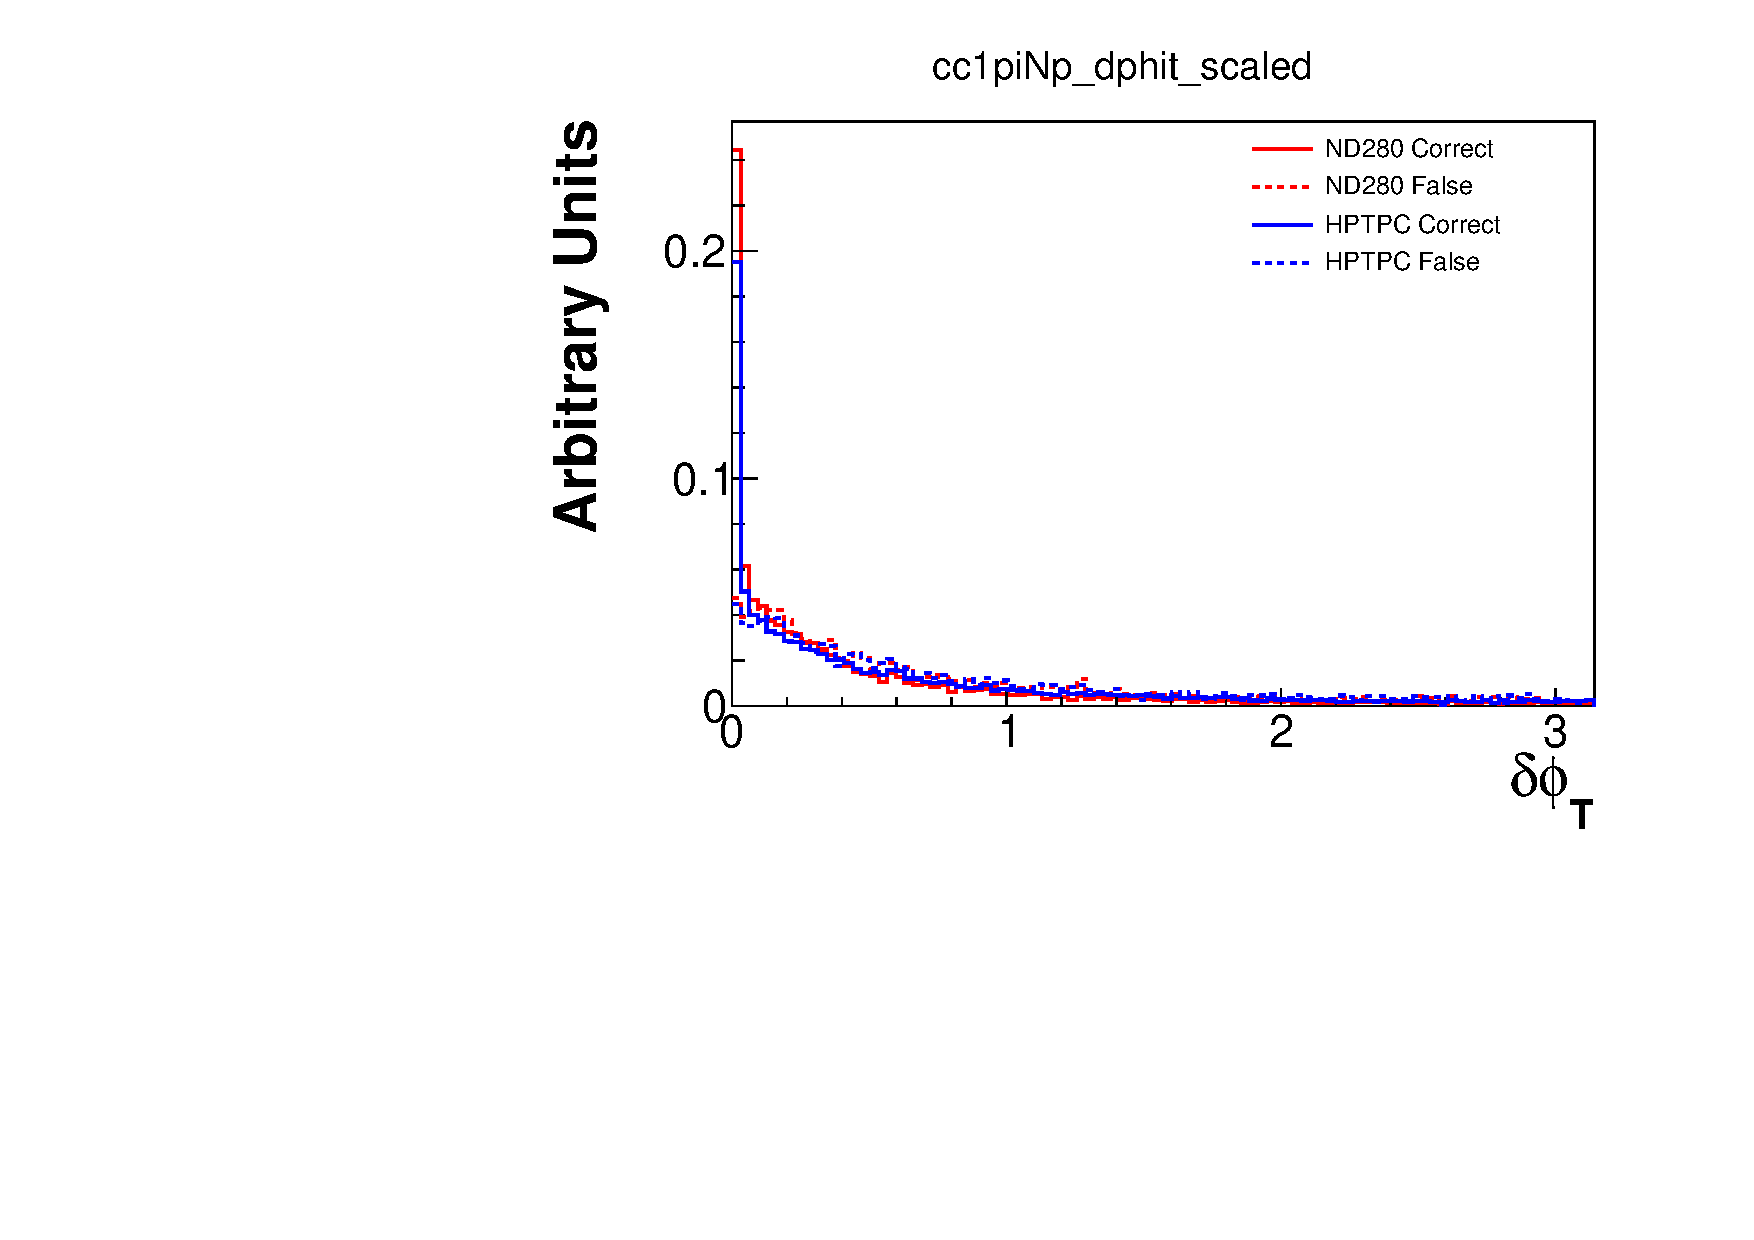
\includegraphics[width=.47\textwidth]{TalkPics/STVforHPTPC_101016/plots/cc1piNp_dphit_scaled.pdf}

    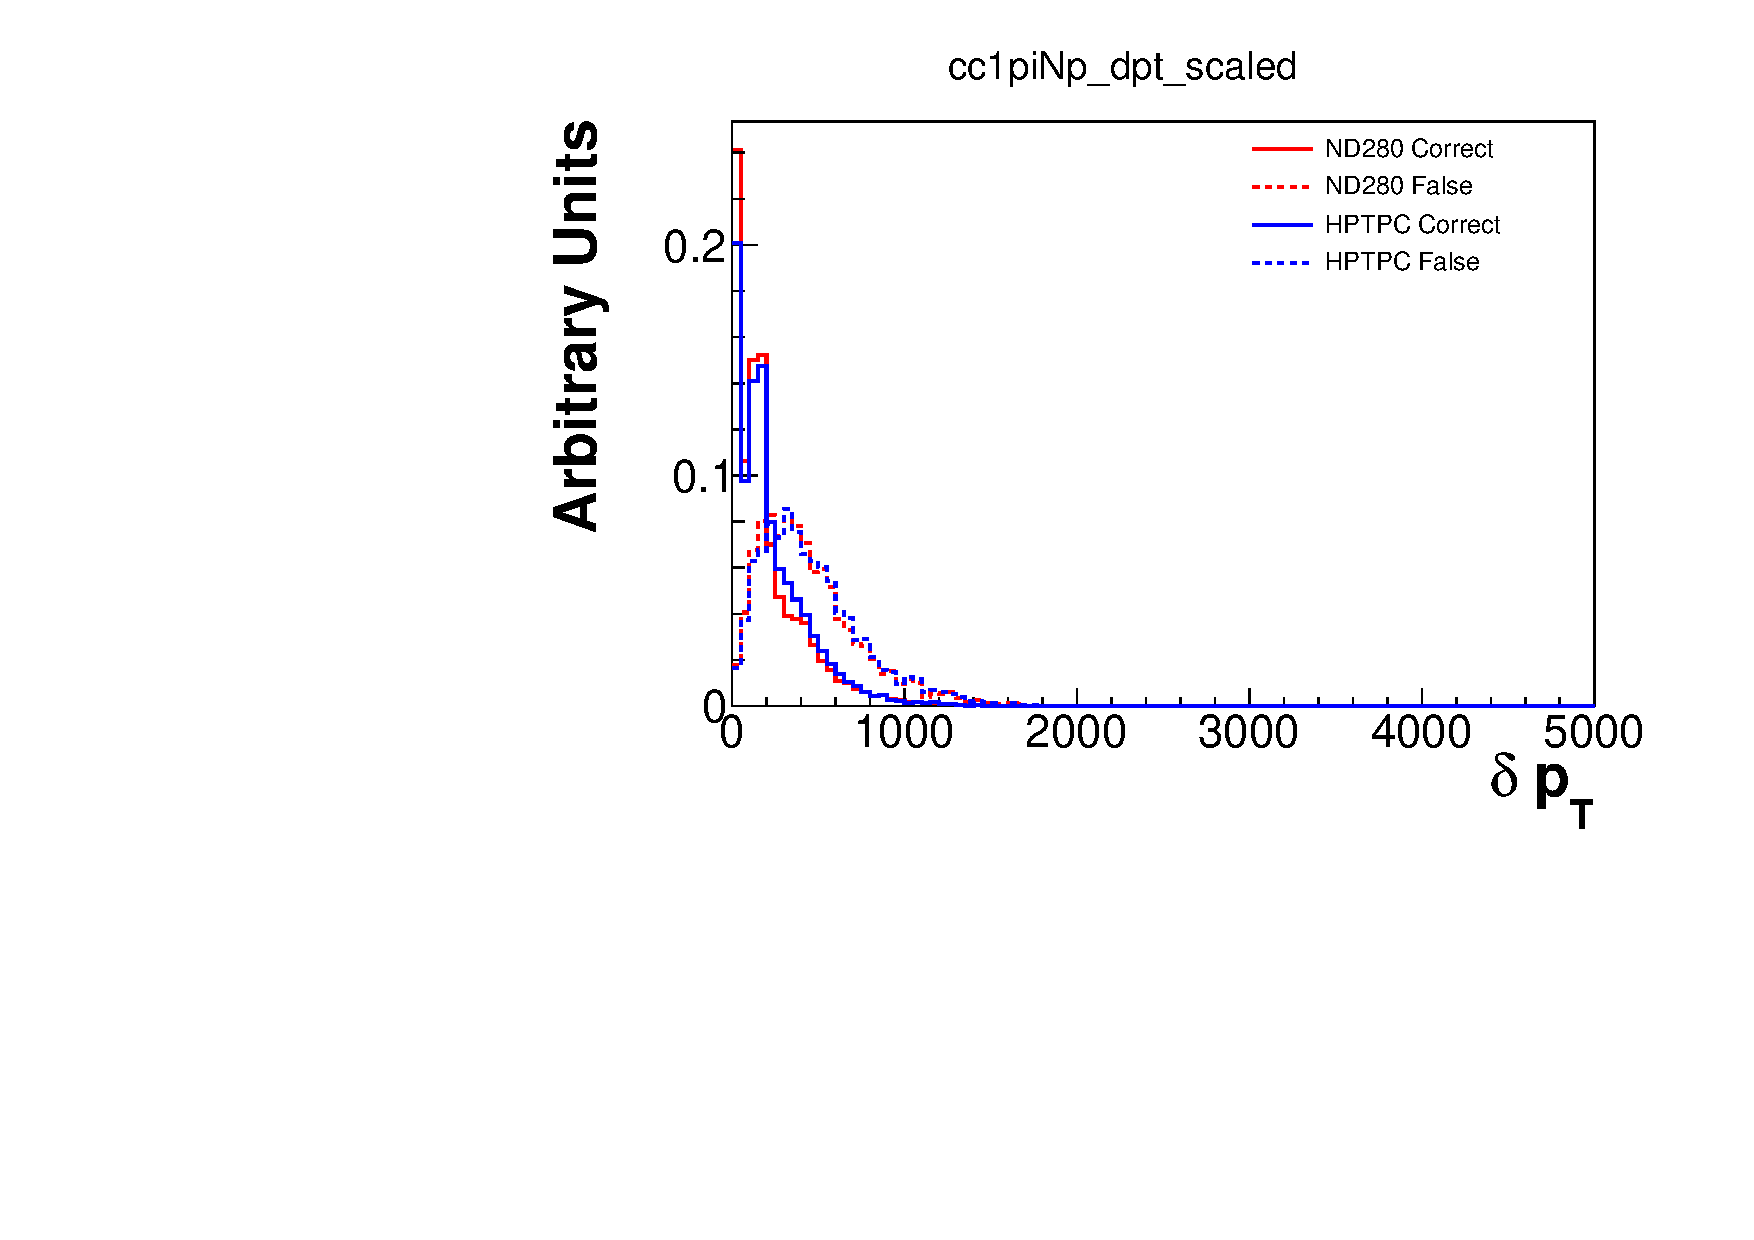
\includegraphics[width=.47\textwidth]{TalkPics/STVforHPTPC_101016/plots/cc1piNp_dpt_scaled.pdf}
  \end{frame}

  \begin{frame}
    \frametitle{}
    \label{lastframe}
    \begin{block}{}
      \begin{itemize}
      \item Transverse variables appear similarly distributed for ND280 and HPTPC thresholds
      \item Exception is CC1$\pi$0p where $\delta p_{T}$ of false events is higher in HPTPC than ND280
      \item[-] Likely caused by there being more low energy pions identified giving a larger difference between lepton and pion momentum
      \item[-] Potentially could be used to separate signal and background
      \item[-] $\delta p_{T}$ could also be used as a proxy for the missing proton
      \end{itemize}
    \end{block}
  \end{frame}

  %Backup goes here
  
\end{fmffile}
\end{document}

\begin{frame}
\end{frame}
